\documentclass{book}
\usepackage[utf8]{inputenc}
\usepackage{amsmath, amssymb, amsthm, amsfonts, mathtools, graphicx, hyperref, fancyhdr, pgfplots, multirow, array, tikz, indentfirst, setspace, enumitem}
\usetikzlibrary{arrows}
\pgfplotsset{width = 10 cm, compat=1.18}
\usepackage[margin=3cm]{geometry}
\newtheorem{theorem}{Theorem}[section]
\newtheorem{definition}[theorem]{Definition}
\newtheorem{example}[theorem]{Example}
\newtheorem{lemma}[theorem]{Lemma}
\newtheorem{corollary}[theorem]{Corollary}
\newtheorem{proposition}[theorem]{Proposition}
\title{\textbf{Introduction to Mathematical Analysis}}
\author{\Large William He}
\date{}

\begin{document}

\maketitle

\tableofcontents

\frontmatter

\chapter{Preface}
\begin{spacing}{1.5}
    \indent Real Analysis is a field of Mathematics which focuses on the real numbers. Related topics include the construction of the real numbers, real sequences and series, and real functions. The objective of this book is to give an introductory understanding of real analysis. \\
    \indent The first chapter gives a review of the basics functions, the construction of the real numbers and sets, we will also look at some properties of these. These are all the relevant knowledge you need to know before actually dive into some more interesting topics (in my opinion) in the real analysis, such as sequences and series, differentiation, and integration. \\
    \indent You, as a reader might have studied calculus before, which focuses more on applying the techniques to compute stuff. However, in real analysis, we will be tackling calculus in a more rigorous approach. Since this books gives an introduction to real analysis, we will focus on single variable calculus only. We will start the theoretical calculus by first looking at limit and continuity. You will then learn differentiation and integration. Unlike usual calculus course, We will study what it means to differentiate/integrate a single variable function. Which kind of functions are able to differentiate/integrate. Why is the Fundamental Theorem of Calculus is true? How do we prove it? \\
    \indent As an apology to the subject of Mathematics, the integral we will be talking about in this book is not the right integral. We will be looking at a form of Riemann Integral, namely Darboux Integral. The reason we are dealing with such integral is that it is much more easier to understand and handle in giving an introductory understanding of real analysis. And this can give a lot of preparation to students to dive into more advanced real analysis in the future, such as the Lebesgue Integral (which is the right integral).\\
    \indent It is recommended that the readers have a basic understanding of the following,
\end{spacing}
\vspace{-2mm}
\begin{itemize}
        \item Some experiences of proofs
        \item Real numbers, functions, sets
        \item Differentiating and integrating functions such as power, exponential, trigonometric, etc.
        \item Differentiate using product, quotient, chain rule; integrating by parts and by substitution
        \item Fundamental Theorem of Calculus
        \item Maclaurin/Taylor Series
\end{itemize}
\begin{center}
    \textbf{\large Mathematical Notations} \ \\
    \ \\
    \begin{tabular}{c|c|c}
        Sets & Number symbols & Statements \\
        \hline
        $A \cup B$: union & $\mathbb{C}$: complex numbers & $\forall$: for all \\
        $A \cap B$: intersection & $\mathbb{R}$: real numbers & $\exists$: there exists \\
        $A^{c}$: complement & $\mathbb{Q}$: rational numbers & $\implies$: implies \\
        $A \backslash B$: difference & $\mathbb{Z}$: integers & $\iff$: if and only if \\
        $\in$: an element of & $\mathbb{N}$: natural numbers & $\neg$: negation \\
        $\subseteq$: a subset of & $\mathbb{R} \backslash \mathbb{Q}$: irrational numbers & \ \\
        $A \times B$: cartesian product & \ & \ \\
\end{tabular}
\end{center}
\ \\
\indent If you spot any typos, feel free to send corrections to

\begin{center}
    $\mathbf{wenjunwilliam.he@mail.utoronto.ca}$
\end{center}

\mainmatter

\chapter{Preliminaries: Functions, Sets, and Real Numbers}

\section{Functions}
You may heard of a function is just take some random input, it will process the input (for example, perform addition, multiplication, root, power, etc.). In the end, it gives an output. Not quite, at least it is not defined that way in Mathematics. We see function as follows.

\begin{definition}
    A \textbf{function} or a \textbf{map} $f : A \rightarrow B$ is an assignment of each element in A to an element of B. \\
    \indent 1) In this case, we call A as the \textbf{domain}, B as the \textbf{codomain}. \\
    \indent 2) If $x \in A$, we write its functional assignment as $f(x)$
\end{definition}

You can tell that, function is actually an assignment rather than doing some random processing with the input. The way we define it that way is that we can now define a map between A and B with non-number or completely irrelevant elements inside.

\begin{example}
    We can define A = \{MAT157 class\} and B = \{days of the year\}. And we have a function $D : A \rightarrow B$ where D outputs the birthday of each element in A. \\
    \indent D(Alan) = May 22 \\
    \indent D(Joe) = Jan 15 \\
    \indent D(Gemma) = Dec 10, etc.
\end{example}

Before giving another example, we will define what is a power set first.

\begin{definition}
    A \textbf{power set} of A is a set of all the subsets of A. We write it as $P(A)$.
\end{definition}

\begin{example}
    We can define $min : P(\mathbb{N}) \rightarrow \mathbb{N}$ which outputs the smallest element of the set.
    \begin{itemize}
        \item If P is the set of prime numbers, then $min(P) = 2$.
        \item We also have $min(\{ 3^{k} : k \in \mathbb{N} \}) = 1$
    \end{itemize}
\end{example}

\begin{example} \label{Example 1.1.5}
    Define $f : \mathbb{Q} \rightarrow \mathbb{Q}$ by $f \left( \frac{a}{b} \right) = a + b$. Is f a function?
\end{example}

\begin{proof}[Solution]
    By definition that each rational number is mapped into a unique rational number. However, if we take $0.5 \in \mathbb{Q}$, we have $f(0.5) = f(\frac{1}{2}) = 1 + 2 = 3.$ But we also have $f(0.5) = f(\frac{2}{4}) = 2 + 4 = 6$, meaning that 0.5 is not mapped to unique element in $\mathbb{Q}$. So f is not a function.
\end{proof}

As we have seen in Example \ref{Example 1.1.5} that f is not a function. We can also say that f is not well defined. This follows the following definition of a well-defined function.

\begin{definition}
    We say that a function $f : A \rightarrow B$ is \textbf{well-defined} if for any $a, b \in A$, $a = b \implies f(a) = f(b)$. In other words, each element of the domain is only mapped to one and only one element in the codomain. \\
    \textbf{Note:} We will only deal with well-defined functions as we can only find interesting results if we define them properly.
\end{definition}

\begin{example}
     Define $f : \mathbb{Q} \rightarrow \mathbb{Q}$ by $f \left( \frac{a}{b} \right) = a + b$ where $gcd(a, b) = 1$. Is f a function?
\end{example}

\begin{proof}[Solution]
    This is left to the readers as an exercise.
\end{proof}

We now had a basic understanding of functions, we will look at some properties of different functions in the next section, which allows us to come out some interesting results or theorems.

\section{Injectivity and Surjectivity}
In this chapter, we will be talking about what does it mean for a function to be injective and surjective. We will also be looking at some of the consequences of defining those terms.

\begin{definition}
    We say that a function $f : A \rightarrow B$ is \textbf{injective} or \textbf{one-to-one} if whenever $f(a) = f(b) \Rightarrow a = b)$
\end{definition}

Even though the term injective might be unfamiliar to you, but you have probably seen what is one-to-one (you may have learnt the horizontal line test, a way to test whether the function is one-to-one or not. If there is a horizontal line 
 y = c, that "cuts" through the function more than one time, then the function is not one-to-one). In other words, this definition is basically saying that any element in the domain is being mapped to different element in the codomain.

\begin{example} \label{Example 1.2.2}
    Define $f : \mathbb{R} \rightarrow \mathbb{R}$ by $f(x) = x^{2}$. Is this function injective?
\end{example}
\begin{proof}[Solution]
    We have f(-2) = 4 = f(2), therefore it fails to be injective.
\end{proof}

Informally speaking, if you use horizontal line test y = c where c > 0, you will see that the horizontal line will touch the function twice. \\
\indent However, that does not mean any function with $f(x) = x^{2}$ is not injective. Recall that when we define a function, we also need to define its domain and codomain. In Example \ref{Example 1.2.2}, we can restrict the domain of this function to non-negative real numbers only. Now, the function is injective, which is shown in Example \ref{Example 1.2.3}.

\begin{example} \label{Example 1.2.3}
    Define $f : (0, \infty) \rightarrow \mathbb{R}$ by $f(x) = x^{2}$. f is injective.
\end{example}
\begin{proof}
Suppose we have $f(a) = f(b) \Rightarrow a^{2} = b^{2} \Rightarrow a = b$ or $a = -b$ \\
Since $a, b > 0$, $a = b$, as otherwise one of the $a, b$ is negative. Hence, since $a$ and $b$ are arbitrary, we have for all $f(a) = f(b) \Rightarrow a = b$, which is the definition of a function being injective.
\end{proof}

\begin{example}
    Define $f : \mathbb{R} \rightarrow \mathbb{R}$ by $f(x) = x^{3}$. Determine whether f is injective.
\end{example}
\begin{proof}[Solution]
    Suppose for arbitrary $a, b \in \mathbb{R}$
    \begin{align*}
        f(a) & = f(b) \\
        \implies a^{3} & = b^{3} \\
        \implies a^{3} - b^{3} & = 0 \\
        \implies (a - b) \times (a^{2} + ab + b^{2}) & = 0
    \end{align*}
    The above equation gives either $a - b = 0$ or $a^{2} + ab + b^{2} = 0$. Now we just need to show that $a - b = 0$ by proving that $a^{2} + ab + b^{2} \geq 0$, for all $a, b \in \mathbb{R}$ and $a^{2} + ab + b^{2} = 0$ only when $a = b = 0$. The rest is left to the reader as an exercise.
\end{proof}

\begin{example}
    Define $f : \mathbb{R} \rightarrow [-1, 1]$ by $f(x) = \sin(x)$. Is f injective? If yes, provide a proof. If not, provide a counterexample and then restrict the domain so that f is injective (no proofs required).
\end{example}

\begin{proof}[Solution]
    Exercise.
\end{proof}

After we defined injectivity, we would like to know any theorems/propositions we can get from this. One intuitive thing we would like to know is that if two functions are injective, what kind of combination of these two functions is still injective. The combination I am talking about is addition, scalar multiplication and composition.

\begin{proposition}
    If $f : A \rightarrow B$ and $g : B \rightarrow C$ are two injective functions. Then $f + g : A \rightarrow C$ is not necessarily injective.
\end{proposition}

\begin{proof}
    If we define $f : \mathbb{R} \rightarrow \mathbb{R}$ by $f(x) = x$, and g the same as f. We have $(f + g)(x)$ is defined as $(f + g)(x) = f(x) + g(x) = 2x$ which is injective. \\
    If we define $f : \mathbb{R} \rightarrow \mathbb{R}$ by $f(x) = x$, and $g : \mathbb{R} \rightarrow \mathbb{R}$ by $g(x) = -x$. We have $(f + g)(x)$ is defined as $(f + g)(x) = f(x) + g(x) = x - x = 0$ which is not injective. 
\end{proof}
We can see that functions does not preserve injectivity under additions. But what about scalar multiplication?
\begin{proposition}
    If $f : A \rightarrow B$ is injective. Then for any $c \in \mathbb{R}, cf : A \rightarrow B$ is not necessarily injective.
\end{proposition}
You may wonder why I did not say that $cf$ is definitely injective. Although this might be intuitively true, but we tend to forgot the case where c = 0. In fact, we can prove that $cf$ is injective for all non-zero c, and not injective when c = 0. This is left as an exercise for the readers.
\begin{proof}
    Exercise. 
\end{proof}
Now, we would like to see whether injectivity is preserved under composition. Although it might be difficult to think intuitively, when actually trying to write something down, we can see that the proof is quite straightforward.
\begin{proposition}
    If $f : B \rightarrow C$ and $g : A \rightarrow B$ are two injective functions. Then $f \circ g : A \rightarrow C$ is injective.
\end{proposition}
\begin{proof}
    Suppose we have
    \begin{align*}
        f(g(a)) & = f(g(b)) \\
        \implies g(a) & = g(b) \ \ \ \ \ \ [\text{Since f is injective}]\\
        \implies a & = b \ \ \ \ \ \ \ \ \ \ [\text{Since g is injective}]
    \end{align*}
    Thus, $f \circ g$ is injective.
\end{proof}

We now know that if both functions f and g are injective, then its composition is also injective. But what about the converse, i.e. if the composition of f and g is injective, is f, g injective?

\begin{proposition} \label{Proposition 1.2.9}
    Suppose $f : B \rightarrow C$ and $g : A \rightarrow B$ are such that $f \circ g : A \rightarrow C$ is injective, then g is injective, and f does not have to.
\end{proposition}

\begin{proof}
    We have that
    \begin{align*}
        g(a) & = g(b) \\
        \Rightarrow f(g(a)) & = f(g(b)) \\
        \Rightarrow (f \circ g)(a) & = (f \circ g)(b) \\
        \Rightarrow a & = b \ \ \ \ \ \ \ \ \ \ \ \ \ [\text{Since } f \circ g \text{ is injective}]
    \end{align*}
    This is exactly the definition of g being injective. \\
    To prove that f does not have to be injective, we can give a counterexample. \\
    Define $g : [0, \infty) \rightarrow \mathbb{R}$ by $g(x) = \sqrt{x}$, and $f : \mathbb{R} \rightarrow \mathbb{R}$ by $f(x) = x^{2}$. We have $f \circ g : [0, \infty) \rightarrow \mathbb{R}$ where $(f \circ g)(x) = x$ which is injective.
\end{proof}

The above proposition is quite interesting, as not all of the function needs to be injective, in order to make the composition innjective. This proposition is also extremely useful as it gives the following immediate corollary.
\begin{corollary}
    Suppose $f_{1} : A_{1} \rightarrow A_{2}, f_{2} : A_{2} \rightarrow A_{3}, ..., f_{n} : A_{n} \rightarrow A_{n+1}$ are n different functions, for any $n \in \mathbb{N}$. If $f_{1}$ is injective then $(f_{n} \circ f_{n-1} \circ ... \circ f_{1})(x)$ is injective.
\end{corollary}

We will now define a surjective function
\begin{definition}
    Suppose a function $f : A \rightarrow B$. \\
    Given a set $X \subseteq A$, we call the \textbf{image} of S is
    $$f(X) = \{b \in B : \exists x \in X, f(x) = b \} = \{f(x) : x \in X \}$$
    Given a set $Y \subseteq B$, we call the \textbf{pre-image} of Y under f is
    $$f^{-1}(Y) = \{a \in A : f(a) \in Y\}$$
    The \textbf{range} of f is $f(A)$ \\
    We call f is \textbf{surjective} if $f(A) = B$. Or we can say,
    $$\forall b \in B, \exists x \in A, s.t. f(x) = b$$
\end{definition}

\begin{example}
    Define $f : \mathbb{R} \rightarrow \mathbb{R}$ by $f(x) = x^{2}$, show that f is not surjective
\end{example}

\begin{proof}[Solution]
    Take -1 in the codomain. We have no $x \in \mathbb{R}$ such that $f(x) = x^{2} = -1$. Hence f is not surjective.
\end{proof}

We have seen from Example \ref{Example 1.2.3} that we can restrict domain to make a function to be injective. If we want to obtain a surjective function, We can also restrict our codomain as well.

\begin{example}
    Define $f : \mathbb{R} \rightarrow [0, \infty)$ by $f(x) = x^{2}$, show that f is surjective
\end{example}

\begin{proof}[Solution]
    Given any $x \in [0, \infty)$, take $\sqrt{x} \in \mathbb{R}$. We have $f(\sqrt{x}) = \sqrt{x}^{2} = x$. Since x is arbitrary element in the codomain, f is surjective.
\end{proof}

Now, does functions preserve surjectivity under addtion, scalar multiplication and composition?

\begin{proposition}
    \begin{itemize}[itemsep = 0pt]
        \item[(1)] If f and g are surjective functions, then $f + g$ does not have to be surjective.
        \item[(2)] Similarly, if f is surjective, then cf does not have to be surjective for some $c \in \mathbb{R}$.
        \item[(3)] Moreover, if $f : B \rightarrow C$ and $g : A \rightarrow B$ are surjective, then $f \circ g : A \rightarrow C$ is also surjective.
    \end{itemize}
\end{proposition}
\begin{proof}
    For (1) and (2), it is quite easy to came up examples that f + g and cf holds or does not hold surjectivity. For (3), note that the proof of injectivity of $f \circ g$ has a similar argument, and the proof is quite similar. These are left to the readers as an exercise.
\end{proof}

We can see that injective functions and surjective functions have lots of similarities, injectivity/surjectivity tends to hold under composition but not others. Note that for injectivity we also proved that if the composition $f \circ g$ is injective, then g is injective. What about surjectivity. We will see that the result is actually similar as well.

\begin{proposition}
    If $f : B \rightarrow C$ and $g : A \rightarrow B$ are such that $f \circ g$ is surjective, then f is surjective, and g does not have to.
\end{proposition}

\begin{proof}
    If $f \circ g$ is surjective then
    $$\forall c \in C, \exists a \in A, s.t. (f \circ g)(a) = f(g(a)) = c$$
    Take $b = g(a)$. We have
    $$\forall c \in C, \exists b = g(a) \in B, s.t. f(g(a)) = f(b) = c$$
    This is the exact definition of surjectivity.
    Example of g does not have to be surjective is left as an exercise.
\end{proof}

We have now defined functions being injective and surjective. The question is, is there a function that is both injective and surjective. Well, there is, and a lot. We also have another name for functions that are both injective and surjective.
\begin{definition}
    We call that $f : A \rightarrow B$ is \textbf{bijective} if f is injective and surjective.
\end{definition}

\begin{example}
    Examples of bijective functions including
    \begin{itemize}[itemsep = 0pt]
        \item $f : \mathbb{R} \rightarrow \mathbb{R}$ by $f(x) = x$
        \item $g : [0, \pi] \rightarrow [-1, 1]$ by $f(x) = \cos(x)$
        \item $h : (-0.5\pi, 0.5\pi) \rightarrow \mathbb{R}$ by $f(x) = \tan(x)$, etc.
    \end{itemize}
\end{example}

You may wonder reason why we came up these terms, it turns out these definitions are strongly connected to invertibility, and this will be discussed more in the next section.

\section{Invertibility}
You have probably heard of invertible (inverse) functions before. For example, if $f : \mathbb{R} \rightarrow \mathbb{R}$ is defined as $f(x) = x^{3}$, then its inverse is define as $f^{-1} : \mathbb{R} \rightarrow \mathbb{R}$ where $f^{-1}(x) = \sqrt[3]{x}$. However, there are different types of inverses in the field of mathematics, where by defining these inverses in certain way, we can find a relationship between these inverses and injectivity and surjectivity. Before starting to defining these inverses, we will first define some special functions.

\begin{definition}
    Given a set A, a function $f : A \rightarrow B$.
    \begin{itemize}[itemsep = 0pt]
        \item[(1)] The \textbf{identity function} (written as $id_{A}$) is a function $id_{A} : a \rightarrow A$ where for any $a \in A, f(a) = a$. 
        \item[(2)] We call f is \textbf{left-invertible} if there exists a function $g : B \rightarrow A$ such that $g \circ f = id_{a}$. Meaning, for all $a \in A, g(f(a)) = a$
        \item[(3)] We call f is \textbf{right-invertible} if there exists a function $g : B \rightarrow A$ such that $f \circ g = id_{a}$. Meaning, for all $b \in B, f(g(b)) = b$
        \item[(4)] We call f is \textbf{invertible} if it is both left-invertible and right-invertible.
    \end{itemize}
\end{definition}

You might be wondering why we need to "split" the definition invertible into left and right. Are there any functions that satisfy only one of the invertibility. Well, there are a lot of them.

\begin{example}
    (1) $f : [0, \infty) \rightarrow \mathbb{R}$ by $f(a) = \sqrt{a}$ is left-invertible where $g : \mathbb{R} \rightarrow [0, \infty)$ and $g(b) = b^{2}$. We have for all $a \in [0, \infty), g(f(a)) = a$. \\
    \indent (2) $f : \mathbb{R} \rightarrow [0, \infty)$ by $f(a) = a^{2}$ is right-invertible where $g : [0, \infty) \rightarrow \mathbb{R}$ and $g(b) = \sqrt{b}$. We have for all $b \in [0, \infty), f(g(b)) = b$.
\end{example}

Note that from the above, in the first example, where f is left-invertible, f is injective. Similarly, f is surjective for the second example (when f is right-invertible). This is not a coincidence. We can give another example,

\begin{example}
    (1) Suppose function f is $f : [-1, 1] \rightarrow \mathbb{R}$ where $f(a) = \arcsin(a)$, f is left-invertible where $g : \mathbb{R} \rightarrow [-1, 1]$ and $g(b) = \sin(b)$ for all $a \in [-1, 1], g(f(a)) = a$. \\
    \indent (2) f is $f : \mathbb{R} \rightarrow [-1, 1]$ where $f(a) = \sin(a)$, f is right-invertible where $g : [-1, 1] \rightarrow [-0.5\pi, 0.5\pi]$ and $g(b) = \arcsin(b)$ for all $b \in [-1, 1], f(g(b)) = b$.
\end{example}

From the above examples, we can see that injectivity is relative to left-invertibility and not the other. Similar argument we can give for surjectivity. Now we can try to prove that they are actually related.

\begin{proposition}
    \begin{itemize}[itemsep = 0pt]
        \item[(1)] A function $f : A \rightarrow B$ is injective if and only if it is left-invertible.
        \item[(2)] A function $f : A \rightarrow B$ is surjective if and only if it is right-invertible.
    \end{itemize}
\end{proposition}

\begin{proof}
    \begin{itemize}[itemsep = 0pt]
        \item[(1)] ($\Rightarrow$) We define g as follows
        \begin{align*}
            g(b) = 
            \begin{cases}
                a & \text{ if f(a) = b} \\
                \hat{a} & \text{ if there is no } a \in A \text{ such that f(a) = b} 
            \end{cases}
        \end{align*}
        Describe g verbally. Since we have f assigns $a \in A$ to $b \in B$, we have if there is f(a) = b, then the function of g basically assigns b back the value of a. For cases such that $f(a) \neq b$ for any $a \in A$, we assign g(b) to a random value in A. We know that g is well-defined (i.e. no g(b) maps to more than one value) because f is injective. Hence, there is only one $a \in A$ such that $f(a) = b$.
        In this case, we have for any $a \in A$, g(f(a)) = a by the way we defined g. \\
        ($\Leftarrow$) Suppose we have
        \begin{align*}
            f(a_{1}) & = f(a_{2}) \\
            \implies f^{-1}(f(a_{1})) & = f^{-1}(f(a_{2})) \\
            \implies a_{1} & = a_{2}
        \end{align*}
    \item[(2)] ($\Rightarrow$) We define g as follows
        \begin{align*}
            g(b) = 
            \begin{cases}
                a & \text{ if only } a \in A \text{ satisfies f(a) = b} \\
                a_{0} & \text{ if } a_{0}, ... a_{n} \text{ satisfies } \forall a_{i}, f(a_{i}) = b
            \end{cases}
        \end{align*}
        Generally speaking, by the surjectivity of f, we know that all elements in b can be written as some f(a). If there is one $a \in A$ where f(a) = b, for function g we can basically assign b back to a, as this is well-defined. In the case where multiple elements $a_{i}$ in A satisfies $f(a_{i}) = b$, we can simply map g from b to one of the $a_{i}$ to keep the function to be well-defined.
        In this case, we have for any $b \in B$, f(g(b)) = b by the way we defined g. \\
        ($\Leftarrow$) Suppose f is left-invertible, then there is a function $g : B \rightarrow A$ such that $f \circ g = id_{B}$ for any $b \in B$. Given any $b \in B$, we can take $g(b) \in A$ which satisfies that $f(g(b)) = b$. Hence, f is surjective.
    \end{itemize}
\end{proof}

These useful results gives an immediate corollary to bijective functions.

\begin{corollary}
    A function $f : A \rightarrow B$ is bijective if and only if it is invertible.
\end{corollary}

\begin{proof}
    Exercise.
\end{proof}

\section{Cardinality and Countability}
We already know that a set is a collections of objects, where not just numbers, literally any stuff can be stored in a set. In this section, we are going to talk about the cardinality ("size") of the sets, meaning how many objects are there in the set. What makes this topic more interesting is that, we will be dealling with sets with infinity objects. Although we think infinity as "the biggest number", this definition is quite implicit. We will be introducing a much more formal definition of infinity in set theory. Moreover, you will know that "there are different sizes of infinities, and some infinity is bigger than the other infinities".

\begin{definition}
    The \textbf{cardinality} of the set A is the number of elements in A, it is written as $|A|$.
\end{definition}

The above definition is a bit vague, it works fine if A has finitely many objects, but what if A has infinite number of objects? This becomes a problem. Also, if we write the cardinality of an infinite set as a specific number or symbol, then as I said before, there will be different sizes of infinities (just trust me this is true for now, you will find out this later), and this will become a lot annoying to define. Instead, mathematicians are quite intelligent, instead of defining the exact size of the infinity, we will try to compare the infinity to other ones. More importantly, we introduces a definition that compares an infinite set to the set of natural numbers (which acts as an "standard" to compare the infinities).

\begin{definition}
    \begin{itemize}[itemsep = 0pt]
        \item[(1)] If there is an injective map $A \rightarrow B$, then we write $|A| \leq |B|$.
        \item[(2)] If there is a surjective map $A \rightarrow B$, then we write $|A| \geq |B|$.
        \item[(3)] If there is an bijection map $A \rightarrow B$, then we write $|A| = |B|$.
    \end{itemize}
\end{definition}

Informally speaking, $|A| \leq |B|$ means set A has less elements than set B. Similarly, $|A| \geq |B|$ means set A has more elements than set B. And for $|A| = |B|$, we meant set A has the same number of elements than set B. \\
\indent You may wonder why we relate this to injectivity and surjectivity. If we think intuitively, this makes sense based on the nature of injectivity and surjectivity. If there is an injective map from set A to set B, we know that each element in set A is pointed to a different element in set B. Therefore, B must have at least the same number of element as A to achieve injectivity, otherwise there will be more than one elements in A pointing to the same elements in B. \\
\indent On the other hand, if there is a surjective map from set A to set B, then for any element in B, there is at least one element in A that maps to B, so A must have at least the same number of element as B to achieve surjectivity, and in the case when in a surjective function, different elements in A are mapped to the same element in B, we have that A must have more elements than B. \\
\indent We will not be talking much more deeper than this, but you can try to come up with examples for A and B have finite numbers of elements.

\begin{definition}
    \begin{itemize}[itemsep = 0pt]
        \item[(1)] We say that A is \textbf{countable} if $|A| \leq |\mathbb{N}|$.
        \item[(2)] We say that A is \textbf{uncountable} if $|A| > |\mathbb{N}|$.
        \item[(3)] \textbf{Note:} In the rest of this book, we assume that 0 is not a natural number unless this is explicitly mentioned.
    \end{itemize}
\end{definition}

One way to think about this definition is that if A is countable (meaning there is an injective map from set A to $\mathbb{N}$), then we can actually count the elements of A one by one, i.e. we can number the elements as 1, 2, 3, ... Although the counting will never end for infinite sets, as long as we are able to count them in such a way, each element in this infinite set will be assigned to one natural number (meaning it will eventually be called). If the set is uncountable, we are not able to count in a way, no matter how we count them, there is always at least one element will never be counted.

After finishing this, we will now look at some counter-intuitive but fasinating result. We will first start by proving that "the set of natural numbers have the same number of elements as the set of even natural numbers". Note that I quoted this claim, as this is not a rigorous way of saying this. Expressing this statement more formally, we have

\begin{example}
    Let $2 \mathbb{N} = \{2, 4, 6, ...\}$ be the set of even natural numbers. Then $|\mathbb{N}| = |2 \mathbb{N}|.$
\end{example}

\begin{proof}
    We define $f : \mathbb{N} \rightarrow 2 \mathbb{N}$ by $f(n) = 2n$. We just need to check whether f is bijective. \\
    We have
    \begin{align*}
        f(a) & = f(b) \\
        \implies 2a & = 2b \\
        \implies a & = b
    \end{align*}
    So f is injective. \\
    For any $n \in 2 \mathbb{N}$, take $\frac{n}{2} \in \mathbb{N}$, we have $f\left(\frac{n}{2}\right) = n.$ So f is surjective. \\
    Hence, f is bijective, and $|\mathbb{N}| = |2 \mathbb{N}|$.
\end{proof}

\begin{example} \label{Example 1.4.5}
    \begin{itemize}[itemsep = 0pt]
        \item[(1)] $|\mathbb{N}|$ = $|\mathbb{N} \cup \{0\}|$
        \item[(2)] Let $S = \{ \frac{1}{2^{k}} : k \in \mathbb{N} \}$, then $|S| = |\mathbb{N}|$
        \item[(3)] $|\mathbb{Z}| = |\mathbb{N}|$.
        \item[(4)] $|\mathbb{N}| = |\mathbb{N} \times \mathbb{N}|$ (Hint: use the Fundamental Theorem of Arithmetic (FTA))
    \end{itemize}
\end{example}

\begin{proof}
    (1), (2) are left to the readers as an exercise.
    \begin{itemize}[itemsep = 0pt]
        \item[(3)] We define $f : \mathbb{Z} \rightarrow \mathbb{N}$ by
        \begin{align*}
            f(x) = 
            \begin{cases}
                2x & \text{ if } x > 0 \\
                1 - 2x & \text{ if } x \leq 0
            \end{cases}
        \end{align*}
        This is bijective, the checking is left for the readers.
        \item[(4)] Define $f : \mathbb{N} \times \mathbb{N} \rightarrow \mathbb{N}$ by $f(x, y) = 2^{x - 1}(2y - 1)$. If $f(x_{1}, y_{1}) = f(x_{2}, y_{2})$, then $2^{x_{1} - 1}(2y_{1} - 1) = 2^{x_{2} - 1}(2y_{2} - 1)$, and by FTA, $x_{1} = x_{2}, y_{1} = y_{2}$, showing injectivity. \\
        For surjectivity, suppose $n \in N$, n can be expressed as a product of prime numbers. Since 2 is the only even prime number, we can split the expression of the product into $2^{x}(2y - 1) = f(x, y)$, where $2^{x}$ is the power of 2 in the expression of n, $2y - 1$ is the product of all the odd prime numbers in the expression. And this is surjective. Hence, this function is bijective.
    \end{itemize}
\end{proof}

Proving whether a specific set is countable or not isn't everything. Very often, theorems and propositions produced in Mathematics works for generalised objects. For example, in cardinality, we have a result of

\begin{theorem} \label{Theorem 1.4.6}
    A countable union of countable sets is countable. \\
    That is, if $S = A_{i} : i \in I$, where $|I| \leq |\mathbb{N}|$, and each $A_{i}$ is a set where $|A_{i}| \leq |\mathbb{N}|$. Then
    $$\bigcup_{i \in I} A_{i} \leq |\mathbb{N}|$$
\end{theorem}

\begin{proof}
    Since $|I| \leq |\mathbb{N}|$, there exists an injection $g : I \rightarrow \mathbb{N}$. Similarly, there exists an injection $f_{i} : A_{i} \rightarrow \mathbb{N}, \forall i \in I.$ \\
    Now, define $h : \bigcup_{i \in I} A_{i} \rightarrow \mathbb{N}$ by $h(a) = 2^{g(n)} 3^{f_n(a)}$, where $a \in A_{n}$. This is injective by the fundamental theorem of arithmetic.
\end{proof}

\begin{example}
    Try to prove Example \ref{Example 1.4.5} Q(3), Q(4) again using Theorem \ref{Theorem 1.4.6}. Exercise.
\end{example}

Currently, we have only learned to find a bijection between two sets to prove they have the same cardinality. But in some cases, it is hard to find one, then is there any other ways to prove them. Actually there is, and this is a really useful theorem and can be easily applied.

\begin{theorem}[Cantor-Schroder-Berstein] \label{Theorem 1.4.8}
    If A, B are two sets such that $|A| \leq |B|$ and $|A| \geq |B|$ then $|A| = |B|$.
\end{theorem}

\begin{proof}
    The proof of this theorem is too technical so that it is beyond the scope. So from now on, we can simply assume this is true. \\
    Note: do not think that this is trivial because we have $|A|$ satisfies $\leq$ and $\geq$ $|B|$ then obviously $|A| = |B|$. This might be trivial in the case we think $|A|$ and $|B|$ as numbers, but we are dealing with sets now. Moreover, putting two vertical lines on both sides does not automatically means we refer $|A|$ and $|B|$ as numbers. In fact, this is just the way we write them for simplicity, and it is not for we can simply assume that they are numbers.
\end{proof}

By using Cantor-Schroder-Berstein (CSB), we can prove that the cardinality of the set of rationals is in fact, the same as the cardinality of the set of natural numbers. Isn't that interesting, it really seems that there are infinitely more rational numbers than the natural numbers, but they still have "equal" number of elements.
\begin{example}
    $|\mathbb{N}| = |\mathbb{Q}|$
\end{example}

\begin{proof}
    $|\mathbb{N}| \leq |\mathbb{Q}|$ is straightforward. \\
    For $|\mathbb{N}| \geq |\mathbb{Q}|$, define $f : \mathbb{Q} \rightarrow \mathbb{N} \times \mathbb{Z}$ by $f(\frac{m}{n}) = (m, n), \text{ where } gcd(m,n) = 1, n \neq 0$. This is an injective function (the checking is left to the readers). Hence, $|\mathbb{Q}| \leq |\mathbb{N} \times \mathbb{Z}|$. And by Theorem \ref{Theorem 1.4.6}, $|\mathbb{N} \times \mathbb{Z}| = \mathbb{N}$, there exists a bijection $g : \mathbb{N} \times \mathbb{Z} \rightarrow \mathbb{N}$. Therefore, by Proposition \ref{Proposition 1.2.9}, we have an injective function $f \circ g : \mathbb{Q} \rightarrow \mathbb{N}$, and so $|\mathbb{N}| \geq |\mathbb{Q}|$. Hence, by Theorem \ref{Theorem 1.4.8}, $|\mathbb{N}| = |\mathbb{Q}|$.
\end{proof}

What about the reals? You might ask. Does the set of real numbers still have the same cardinality of the set of natural numbers? Well, actually no. And I will now prove it.

\begin{proposition}
    $|\mathbb{R}| > |\mathbb{N}|$.
\end{proposition}

\begin{proof}
    $|\mathbb{R}| \geq |\mathbb{N}|$ is straightforward. \\
    To prove that $|\mathbb{R}| > |\mathbb{N}|$, it is enough to prove that $|(0, 1)| > |\mathbb{N}|$ (check, try to find a bijection between $(0, 1)$ and $\mathbb{R}$ by using one of the trignometric function). \\
    Suppose for a contradiction that $(0, 1) = \mathbb{N}$, then there exists a bijection $f \circ \mathbb{N} \rightarrow (0, 1)$ where we can write \\
    \indent $f(1) = 0.a_{11}a_{12}a_{13}...$ \\
    \indent $f(2) = 0.a_{21}a_{22}a_{23}...$ \\
    \indent $f(3) = 0.a_{31}a_{32}a_{33}...$ \\
    where $a_{ij}$ is the jth decimal of f(i). \\
    Now define a real number $b = 0.b_{1}b_{2}b_{3}...$ where
    \begin{align*}
        b_{i} =
        \begin{cases}
            0 & \text{if } a_{ii} = 1 \\
            1 & \text{otherwise}
        \end{cases}
    \end{align*}
    Note by construction, $b \neq f(i), \forall i \in \mathbb{N}$, as b differs f(i) by exactly one decimal (which is the ith decimal). So, contradiction that f is a bijection. And $|\mathbb{N}| = |(0, 1)| > |\mathbb{N}|$
\end{proof}

\section{Arithmetics of the Real Numbers}
We are now going to talk about real numbers, and how they are constructed. You may already had a basic understandings of real numbers. We can come up with lots of examples of real numbers, 1, -2049, 0.4, $\pi$, $\sqrt{2}$, 23952.930834, etc. In this section, we are not going to define what the real numbers are. Instead we are going to find how real numbers behave. We will start by stating some axioms of the real number. All Maths is created by assuming some basic axioms that we think are intuitively true. They acts as a source (base) and we try to build more theorems/results on top of our axioms. Axioms are very important in the field of Mathematics, if the axioms break, then all the theorems we found in these thousands of years will suddenly become garbage. Therefore, keeping our axiom correct is really essential. \\
Our axioms of arithmetics includes
\begin{itemize}
    \item For $a, b \in \mathbb{R}$, there exists a unique real number $a + b$ called their \textbf{sum}.
    \item For $a, b \in \mathbb{R}$, there exists a unique real number $a \cdot b$ called their \textbf{product}.
\end{itemize}

For $a, b, c \in \mathbb{R}$

\begin{itemize}[itemsep = 0pt]
    \item Addition and multiplication is \textbf{commutative}. That is, $a + b = b + a$ and $a \cdot b = b \cdot a$
    \item Addition and multiplication is \textbf{associative}. That is, $a + (b + c) = (a + b) + c$ and $a \cdot (b \cdot c) = (a \cdot b) \cdot c$
    \item For all $a \in \mathbb{R}$, there exists a unique real number $-a$ called the \textbf{additive inverse} or its negative that satisfies $a + (-a) = 0$.
    \item For all $a \in \mathbb{R}, a \neq 0$, there exists a unique real number $a^{-1}$ called the \textbf{multiplicative inverse} or its reciprocal that satisfies $a \cdot a^{-1} = 1$.
    \item There exists a special element $0 \in \mathbb{R}$ called the \textbf{additive identity} or zero that satisfies for all $a \in \mathbb{R}, a + 0 = a$.
    \item There exists a special element $1 \in \mathbb{R}$ called the \textbf{multiplicative identity} or one that satisfies for all $a \in \mathbb{R}, a \cdot 1 = a$.
    \item Multiplication is \textbf{distributive} over addition. That is, $a \cdot (b + c) = a \cdot b + a \cdot c$
    \item To avoid total collapse of the field of Mathematics, $0 \neq 1$
\end{itemize}

Note that last axiom is extremely obvious, but without that, we cannot prove some useful results (which you will see very soon).\\
Now some of your may realise this is the field axiom. As an extension, I will talk about what is a field. \\
Moreover, all the axioms are about addition and multiplication, but what about subtraction and division. Apparently, we will not be dealing with subtraction and division, as we typically view these operations as adding the \textbf{additive inverse} and mulitplying the \textbf{multiplicative inverse}.

\begin{definition}
    A set $\mathbb{F}$ with operations of addition and multiplication that satisfies all the above axioms is called a \textbf{field}.
\end{definition}

\begin{example}
    We just talked about $\mathbb{R}$, which we said is a field. Similarly, $\mathbb{Q}$ is a field. However, $\mathbb{Z}$ is not a field, as not every non-zero element in $\mathbb{Z}$ has a multiplicative inverse.
\end{example}

You might wonder what results can we come up with after coming up with these axioms. Luckily, you don't need to find these, as people have done it in the past! But what is more interesting is the way they prove these result. The proof are quite easy to follow. Therefore, I will leave some of them as an exercise for you.

\begin{proposition} \label{Proposition 1.5.3}
    Let a, b, c, x, y be real numbers.
    \begin{itemize}[itemsep = 0pt]
        \item[(1)] If $a + x = a$ for all $a$ then $x = 0$.
        \item[(2)] If $a \cdot x = a$ for all $a$ then $x = 1$.
        \item[(3)] If $a + x = a + y$ then $x = y$.
        \item[(4)] If $a \neq 0$ and $a \cdot x = a \cdot y$ then $x = y$.
        \item[(5)] $-(-a) = a$.
        \item[(6)] If $a \neq 0$ then $\frac{1}{\frac{1}{a}} = a$.
        \item[(7)] For all $a \in \mathbb{R}, a \cdot 0 = 0$.
        \item[(8)] $-(a + b) = (-a) + (-b)$.
        \item[(9)] $a \cdot (-b) = -(a \cdot b)$. This result gives that $(-1) \cdot a = -a$.
        \item[(10)] $(a + b) \cdot c = a \cdot c + b \cdot c$.
        \item[(11)] $-0 = 0$.
        \item[(12)] $(-1) \cdot (-1) = 1$.
        \item[(13)] If $a \cdot b = 0$ then $a = 0$ or $b = 0$. If $a \neq 0$ and $b \neq 0$ then $(a + b)^{-1} = a^{-1} \cdot b^{-1}$.
    \end{itemize}
\end{proposition}

\begin{proof}
    \begin{itemize}[itemsep = 0pt]
        \item[(1)] We have
        \begin{align*}
            x & = x + 0 \ \ \ \ [\text{additive identity}] \\
            & = 0 + x \ \ \ \ [+ \text{ is commutative}] \\
            & = 0 \ \ \ \ [0 + x = 0 \text{ by hypothesis}]
        \end{align*}
        \item[(2)] This is similar to (1), we leave this as an exercise.
        \item[(3)] We have
        \begin{align*}
            x & = x + 0 \ \ \ \ [\text{additive identity}] \\
            & = x + (a + (-a)) \ \ \ \ [\text{additive inverse}] \\
            & = (x + a) + (-a) \ \ \ \ [+ \text{is associative}] \\
            & = (a + x) + (-a) \ \ \ \ [+ \text{is commutative}] \\
            & = (a + y) + (-a) \ \ \ \ [\text{by hypothesis}] \\
            & = (y + a) + (-a) \ \ \ \ [+ \text{is commutative}] \\
            & = y + (a + (-a)) \ \ \ \ [+ \text{is associative}] \\
            & = y + 0 \ \ \ \ [\text{additive inverse}] \\
            & = y \ \ \ \ [\text{additive identity}]
        \end{align*}
        \item[(4)] This is similar to (3), exercise.
        \item[(5)] We have
        $$(-a) + a = a + (-a) = 0 \ \ \ \ [\text{additive inverse}]$$ \\
        We also know that
        $$(-a) + (-(-a)) = 0 \ \ \ \ [\text{addtive inverse}]$$ \\
        Therefore,
        $$(-a) + (-(-a)) = (-a) + a \implies (-(-a)) = a \ \ \ \ [\text{by (3)}]$$
        \item[(6)] This is similar to (5), exercise.
        \item[(7)] We have
        $$a \cdot (0 + 0) = a \cdot 0 + a \cdot 0 \ \ \ \ [\cdot \text{ is distribute over } +]$$ \\
        We also have
        \begin{align*}
            a \cdot (0 + 0) & = a \cdot 0 \ \ \ \ [\text{additive identity}] \\
            & = a \cdot 0 + 0 \ \ \ \ [\text{addtive identity}]
        \end{align*}
        And so
        $$a \cdot 0 + a \cdot 0 = a \cdot 0 + 0 \implies a \cdot 0 = 0 \ \ \ \ [\text{by (3)}]$$
        \item[(8)] We have
        $$(a + b) + (-(a + b)) = 0 \ \ \ \ [\text{additive inverse}]$$
        We also know that
        \begin{align*}
            (a + b) + ((-a) + (-b)) & = (a + b) + ((-b) + (-a)) \ \ \ \ [+ \text{ is commutative}] \\
            & = ((a + b) + (-b)) + (-a)) \ \ \ \ [+ \text{ is associative}] \\
            & = (a + (b + (-b)) + (-a)) \ \ \ \ [+ \text{ is associative}] \\
            & = (a + 0) + (-a) \ \ \ \ [\text{additive inverse}] \\
            & = a + (-a) \ \ \ \ [\text{additive identity}] \\
            & = 0 \ \ \ \ [\text{additive identity}] \\
        \end{align*}
        Finally, we have
        $$(a + b) + (-(a + b)) = (a + b) + ((-a) + (-b)) \implies -(a + b) = (-a) + (-b) \ \ \ \ [\text{by (3)}]$$
        \item[(9)] We have
        \begin{align*}
            a \cdot b + a \cdot (-b) = a \cdot (b + (-b)) \ \ \ \ [\cdot \text{ is distributive over } +] \\
            = a \cdot 0 \ \ \ \ [\text{multiplicative inverse}]
        \end{align*}
        We also know that
        $$a \cdot b + (-(a \cdot b)) = 0 \ \ \ \ [\text{additive inverse}]$$
        Therefore,
        $$a \cdot b + a \cdot (-b) = a \cdot b + (-a(a \cdot b)) \implies a \cdot (-b) = -(a \cdot b) \ \ \ \ [\text{by (3)}]$$
        \item[(10)] We have
        \begin{align*}
            (a + b) \cdot c & = c \cdot (a + b) \ \ \ \ [\cdot \text{ is commutative}] \\
            & = c \cdot a + c \cdot b \ \ \ \ [\cdot \text{ is distributive over } +] \\
            & = a \cdot c + c \cdot b \ \ \ \ [\cdot \text{ is commutative}] \\
            & = a \cdot c + b \cdot c \ \ \ \ [\cdot \text{ is commutative}] 
        \end{align*}
        Note: This result is a bit different to the distributivity of multiplication over addition axiom (you can check). So we cannot use this axiom directly.
        \item[(11)] We have
        $$0 + 0 = 0 \ \ \ \ [\text{additive identity}]$$
        We also have
        $$0 + (-0) = 0 \ \ \ \ [\text{additive inverse}]$$
        Thus,
        $$0 + (-0) = 0 + 0 \implies -0 = 0 \ \ \ \ [\text{by (3)}]$$
        \item[(12)] We have
        \begin{align*}
            (-1) + (-1) \cdot (-1) & = (-1) \cdot 1 + (-1) \cdot (-1) \ \ \ \ [\text{multiplicative inverse}] \\
            & = (-1) \cdot (1 + (-1)) \ \ \ \ [\cdot \text{ is distributive over } +] \\
            & = (-1) \cdot 0 \ \ \ \ [\text{additive inverse}] \\
            & = 0 \ \ \ \ [\text{by (7)}] \\
        \end{align*}
        We also know that
        \begin{align*}
            (-1) + (-(-1)) & = (-1) + 1 \ \ \ \ [\text{by (5)}] \\
            & = 1 + (-1) \ \ \ \ [+ \text{ is commutative}] \\
            & = 0 \ \ \ \ [\text{additive inverse}]
        \end{align*}
        \item[(13)] Suppose for a contradiction that $a \neq 0, b \neq 0$ but $a \cdot b = 0$. Then
        \begin{align*}
            0 & = (a^{-1} \cdot b^{-1}) \cdot 0 \ \ \ \ [\text{by (7)}] \\
            & = (a^{-1} \cdot b^{-1}) \cdot (a \cdot b) \ \ \ \ [\text{by hypothesis}] \\
            & = (a^{-1} \cdot b^{-1}) \cdot (b \cdot a) \ \ \ \ [\cdot \text{ is commutative}] \\
            & = \left( (a^{-1} \cdot b^{-1}) \cdot b \right) \cdot a \ \ \ \ [\cdot \text{ is associative}] \\
            & = \left( a^{-1} \cdot (b^{-1} \cdot b) \right) \cdot a \ \ \ \ [\cdot \text{ is associative}] \\
            & = \left( a^{-1} \cdot 1) \right) \cdot a \ \ \ \ [\text{multiplicative inverse}] \\
            & = a^{-1} \cdot a \ \ \ \ [\text{multplicative identity}] \\
            & = a \cdot a^{-1} \ \ \ \ [\cdot \text{ is commutative}] \\
            & = 1 \ \ \ \ [\text{multiplicative inverse}]
        \end{align*}
        Contradiction to the axioms. \\
        We have that
        \begin{align*}
            (a \cdot b) \cdot (a^{-1} \cdot b^{-1}) & = (a^{-1} \cdot b^{-1}) \cdot (a \cdot b) \ \ \ \ [\cdot \text{ is commutative}] \\
           & = 1 \ \ \ \ [\text{from previously}]
        \end{align*}
        We also have
        $$(a \cdot b) \cdot (a + b)^{-1} = 1 \ \ \ \ [\text{multiplicative inverse}]$$
        Thus
        $$(a \cdot b) \cdot (a + b)^{-1} = (a \cdot b) \cdot (a^{-1} \cdot b^{-1}) \implies (a + b)^{-1} = a^{-1} \cdot b^{-1} \ \ \ \ [\text{by (3)}]$$
    \end{itemize}
\end{proof}

Note that in this proof, I showed as many steps as possible, this is just to let you keep track on my thought process, so that you are more familiar with the concepts. In future proofs, without affecting logical process, for simplicity, I will skip some steps.
You might be wondering why we need to prove these results even it seems to be very intuitive and "trivial". Why not put them as the axiom as well? But that is the beauty of Mathematics, we would like to keep the accuracy and rigour of our work high, we would always try to have as less axioms as possible while still be able to prove a lot of stuff. Having less axioms are able to increase our rigour as it shows our theorems and other results are not that dependent as the one that is supported by less axioms. \\
From now on, we have know that how real numbers behave in addition and multiplication, what about powers.

\begin{definition}
    For any $a \in \mathbb{R} \backslash \{ 0 \}, a^{0} = 1$. \\
    We also define powers inductively. That is, for $k \geq 0, k \in \mathbb{Z}, a^{k + 1} = a^{k} \cdot a$. \\
    For $k < 0, k \in \mathbb{Z}, a^{k} = \frac{1}{a^{-k}}$
\end{definition}

\begin{lemma}
    For all $a \in \mathbb{R} \backslash \{ 0 \}$, for all $m, n \in \mathbb{Z}, a^{m + n} = a^{m}a^{n}$.
\end{lemma}

\begin{proof}
    We can prove inductively on n. \\
    Base case: When n = 0
    \begin{align*}
        a^{m + n} & = a^{m + 0} \ \ \ \ [n = 0] \\
        & = a^{m} \ \ \ \ [\text{additive identity}] \\
        & = a^{m} \cdot 1 \ \ \ \ [\text{multiplicative identity}] \\
        & = a^{m} \cdot a^{0} \ \ \ \ [\text{by definition}] \\
        & = a^{m} \cdot a^{n} \ \ \ \ [n = 0]
    \end{align*}
    Inductive step: Suppose P(k) is true, then $a^{m + k} = a^{m} \cdot a^{k}$ \\
    We have for P(k + 1):
    \begin{align*}
        a^{m + (k + 1)} & = a^{m + k} \cdot a \ \ \ \ [\text{by definition}] \\
        & = (a^{m} \cdot a^{k}) \cdot a \ \ \ \ [\text{by inductive hypothesis}] \\
        & = a^{m} \cdot (a^{k} \cdot a) \ \ \ \ [\cdot \text{ is associative}] \\
        & = a^{m} \cdot a^{k + 1} \ \ \ \ [\text{by definition}]
    \end{align*}
    
    Now, by this induction, we have proved that for all $n \geq 0, n \in \mathbb{Z}$, the Lemma holds. We also need to prove P(k - 1) is true as well. Before do that, we need to know that the definition also gives the following
    
    \begin{align*}
        a^{k} & = a^{k - 1} \cdot a \ \ \ \ [\text{by definition}] \\
        a^{k} \cdot a^{-1} & = a^{k - 1} \cdot a \cdot a^{-1} \ \ \ \ [a^{-1} \text{ exists as } a \neq 0] \\
        a^{k} \cdot a^{-1} & = a^{k - 1} \cdot 1 \ \ \ \ [\text{multiplicative inverse}] \\
        a^{k} \cdot a^{-1} & = a^{k - 1} \ \ \ \ [\text{multiplicative identity}]
    \end{align*}

    Using the above result, we have that
    
    \begin{align*}
        a^{m + (k - 1)} & = a^{(m + k) + (-1)} \ \ \ \ [+ \text{ is associative}] \\
        & = a^{m + k} \cdot a^{-1} \ \ \ \ [\text{by our result}] \\
        & = (a^{m} \cdot a^{k}) \cdot a^{-1} \ \ \ \ [\text{by definition}] \\
        & = a^{m} \cdot (a^{k} \cdot a^{-1}) \ \ \ \ [\text{by definition}] \\
        & = a^{m} \cdot a^{k-1} \ \ \ \ [\text{by our result}]
    \end{align*}
    By two inductions, we have proved that for all $m, n \in \mathbb{Z}, a^{m + n} = a^{m}a^{n}$.
    
\end{proof}

\section{Inequalities of the Real Numbers}
We have just covered how arithmetics behave in the real numbers by stating a list of axioms. Are these axioms enough to find all the results we want? Apparently no, the axioms provided are not able to tell the ordering of the real numbers (how a real number is bigger than the other). In this chapter, we will deal with the inequalities. \\
If we think of real numbers, we normally think of a real number line, where the centre is 0. The portion on the right of the centre is positive, as we go further to the right, the number grows bigger. On the left of the centre we have the negatives, the number grows smaller as we keep going left.

\begin{center}
    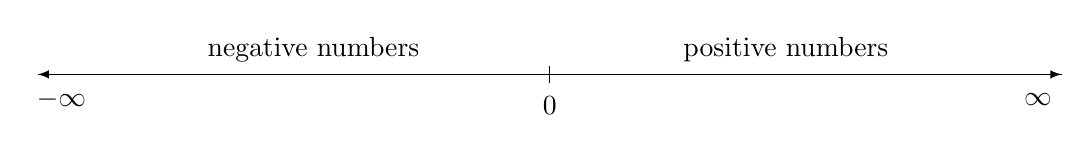
\begin{tikzpicture}
        \draw[latex-] (-6.5,0) -- (6.5,0) ;
        \draw[-latex] (-6.5,0) -- (6.5,0) ;
        \draw[shift={(0,0)},color=black] (0pt,3pt) -- (0pt,-3pt);
        \draw[shift={(0,0)},color=black] (0pt,0pt) -- (0pt,-3pt);
        \node at (0, -0.4) (zero) {0};
        \node at (3, 0.32) (positive) {positive numbers};
        \node at (-3, 0.32) (negative) {negative numbers}; 
        \node at (6.2, -0.32) (infinity) {$\infty$};
        \node at (-6.2, -0.32) (-infinity) {$-\infty$}; 
\end{tikzpicture}
\end{center}

Again we will give all the axioms for ordering. e first look at the set of positive numbers $\mathbb{P}$, where $\mathbb{P} \subseteq \mathbb{R}$, this set satisfies

\begin{itemize}
    \item Closure under addition: meaning if $a, b \in \mathbb{P}$, then $a + b \in \mathbb{P}$
    \item Closure under multiplication: meaning if $a, b \in \mathbb{P}$, then $a \cdot b \in \mathbb{P}$
    \item For any $a \in \mathbb{R}$, either $a \in \mathbb{P}$ or $a = 0$ or $-a \in \mathbb{P}$
\end{itemize}
We also call $\mathbb{P} \cup \{ 0 \}$ as non-negative numbers. \\
We say $a < b$, or $b > a$ when $b - a \in \mathbb{P}$. \\
We say $a \leq b$, or $b \geq a$ when $b - a \in \mathbb{P} \cup \{ 0 \}$. \\
Now by these axioms, we can come up with some interesting results.

\begin{proposition}
    Given any $a, b, c \in \mathbb{R}$
    \begin{itemize}[itemsep = 0pt]
        \item[(1)] $a \leq a$ (Reflexive)
        \item[(2)] If $a \leq b$ and $b \leq a$ then $a = b$ (Anti-symmetric)
        \item[(3)] If $a \leq b$ and $b \leq c$ then $a \leq c$, similarly when we switch the symbol $\leq$ to $<$ (Transitive)
        \item[(4)] Exactly one of the $a < b$ or $a = b$ or $a > b$ holds (Trichotomy)
    \end{itemize}
\end{proposition}

\begin{proof}
    \begin{itemize}[itemsep = 0pt]
        \item[(1)] We have $a - a = 0$ by additive inverse. And $0 \in \mathbb{P} \cup \{ 0 \} \implies a \leq a$.
        \item[(2)] Suppose $a \leq b$ and $b \leq a$, we then have $b - a \in \mathbb{P} \cup \{ 0 \}$ and $a - b \in \mathbb{P} \cup \{ 0 \}$. \\
        If $a - b = 0$ or $b - a = 0$ then $a = b$. \\
        Otherwise, we have $b - a \in \mathbb{P}$ and $a - b \in \mathbb{P}$. But $b - a = -(a - b)$. So, we have $a - b \in \mathbb{P}$ and $-(a - b) \in \mathbb{P}$, contradiction to the axioms.
        \item[(3)] We have
        \begin{align*}
            c - a & = c + 0 - a \\
            & = c + (- b) + b - a \\
            & = (c - b) + (b - a) \\
        \end{align*}
        We know that $b \leq c \implies c - b \in \mathbb{P}$. Similarly $a \leq b \implies b - a \in \mathbb{P}$. By closure under addition, $c - a = (c - b) + (b - a) \in \mathbb{P} \implies a \leq c$.
        \item[(4)] This is the direct consequences from the axiom.
    \end{itemize}
\end{proof}

The next proposition is more useful in the fields of arithmetics and inequalities.

\begin{proposition}
    Suppose $a, b, c \in \mathbb{R}$
    \begin{itemize}[itemsep = 0pt]
        \item[(1)] $0 < 1$
        \item[(2)] If $a < b$ then $a + c < b + c$.
        \item[(3)] If $a < b$ and $0 < c$ then $ac < bc$.
        \item[(4)] $a < b \iff -b < -a$. The direct consequences of this is that $a > 0 \iff -a < 0$.
        \item[(5)] $a^{2} \geq 0$, where $a^{2} = 0 \iff a = 0$.
        \item[(6)] $a > 0 \iff \frac{1}{a} > 0$.
        \item[(7)] If $a, b > 0$ and $a < b$ then $\frac{1}{b} < \frac{1}{a}$.
    \end{itemize}
\end{proposition}

\begin{proof}
    \begin{itemize}[itemsep = 0pt]
        \item[(1)] By trichotomy, either $0 < 1$ or $0 = 1$ or $0 > 1$. But by axiom, $0 \neq 1$, so we just need to prove that $0 \ngtr 1$. \\
        Suppose for a contradiction that $0 > 1$. Then $-1 \in \mathbb{P}$ and so $1 = (-1) \cdot (-1) \in \mathbb{P}$ by closure under multiplication. This gives $0 < 1$, contradiction. So $0 < 1$.
        \item[(2)] We have $a < b \Rightarrow b - a \in \mathbb{P}$. \\
        Then
        \begin{align*}
            (b + c) - (a + c) & = b + c - a - c \\
            & = b - a + c - c \\
            & = b - a + 0 \\
            & = b - a \in \mathbb{P}
        \end{align*}
        This shows that $a + c < b + c$.
        \item[(3)] We have $a < b \rightarrow b - a \in \mathbb{P}$ \\
        We also know that $bc - ac = (b - a) \cdot c$
        Since $b - a \in \mathbb{P}$ and $c \in \mathbb{P}$, $(b - a) \cdot c$ by closure. Hence, $bc > ac$
        \item[(4)] We have
        \begin{align*}
            a < b & \iff b - a \in \mathbb{P} \\
            & \iff - (-b) - a \in \mathbb{P} \\
            & \iff - a - (-b) \in \mathbb{P} \\
            & \iff (-a) - (-b) \in \mathbb{P} \\
            & \iff -a > -b
        \end{align*}
        \item[(5)] By (13), $a = 0 \iff a^{2} = 0$ \\
        If $a \neq 0$, either $a \in \mathbb{P}$ or $-a \in \mathbb{P}$. But either of them would lead to $a^{2} = a \cdot a = (-a) \cdot (-a)$, where one of the $a \cdot a$ or $(-a) \cdot (-a)$ is in $\mathbb{P}$ by closure. Hence $a^{2} \in \mathbb{P}$.
        \item[(6)] Suppose for a contradiction that $a > 0$ and $\frac{1}{a} < 0$, so $a > 0$ and $-\frac{1}{a} > 0$. \\
        Then $-1 = -(a \cdot \frac{1}{a}) = a \cdot (-\frac{1}{a}) > 0$, which contradicts (1).
        Converse is similar for $\frac{1}{a} > 0$ and $a < 0$.
        \item[(7)] We have $a, b > 0 \rightarrow \frac{1}{a}, \frac{1}{b} > 0$ by (6). \\
        Then
        \begin{align*}
            a \cdot \frac{1}{a} \cdot \frac{1}{b} & < b \cdot \frac{1}{a} \frac{1}{b} \ \ \ \ [\text{by (4)}] \\
            \implies 1 \cdot \frac{1}{b} & < 1 \cdot \frac{1}{a} \\
            \implies \frac{1}{b} & < \frac{1}{a}
        \end{align*}
    \end{itemize}
\end{proof}

\section{Modulus of the Real Numbers}

We will then deal with the modulus of the real numbers.

\begin{definition}
    Let $x \in \mathbb{R}$, we define the \textbf{modulus} or \textbf{absolute value} of x (written $|x|$) is
    \begin{align*}
        |x| =
        \begin{cases}
            x & if x > 0 \\
            0 & if x = 0 \\
            -x & if x < 0
        \end{cases}
    \end{align*}
\end{definition}

You may be more familiar with the modulus as the "distance" from x to the origin.

\begin{proposition} \label{Proposition 1.7.2}
    \begin{itemize}[itemsep = 0pt]
        \item[(1)] $|a| \geq 0$.
        \item[(2)] $|-a| = |a|$.
        \item[(3)] $-|a| \leq a \leq |a|$.
        \item[(4)] $|a|^{2} = a^{2}$.
        \item[(5)] $|ab| = |a||b|$.
        \item[(6)] Let $b \geq 0$, we have $|a| < b \iff -b < a < b$. Similarly if $<$ is swapped by $\leq$.
    \end{itemize}
\end{proposition}

\begin{proof}
    \begin{itemize}[itemsep = 0pt]
        \item[(1)] For $a > 0$, use closure. For $a = 0$, straightforward. For $a < 0$, use $(-a)(-a) = a^{2}$, exercise.
        \item[(2)] For $a = 0, a < 0$, straightforward. For $a > 0$, use $-(-a) = a$, exercise.
        \item[(3)] Exercise.
        \item[(4)] For $a > 0, a = 0$, straightforward. For $a < 0$, use $(-a) \cdot (-a) = a^{2}$, exercise.
        \item[(5)] If $a \geq 0, -|a| \leq 0 \leq a = |a|$. \\
        If $a < 0, -|a| = a \leq 0 \leq |a|$.
        \item[(6)] $(\Rightarrow)$ Suppose that $|a| < b$, by (3), $-b < -|a| < a < |a| < b$. \\
        $(\Leftarrow)$ Suppose that $-c < a < c \implies -a < c \text{ and } a < c$. And since $|a| = a$ or $-a$, so $|a| < c$.
    \end{itemize}
\end{proof}
These results aren't all of them, we are now going to look at the triangle inequality which is one of the most important results and widely used in a lot of areas such as geometry and of course the topic we are dealing with in this book, Analysis!
\begin{theorem}[Triangle Inequality]
    For any $a, b \in \mathbb{R}$
    \begin{itemize}[itemsep = 0pt]
        \item[(1)] $|a + b| \leq |a| + |b|$.
        \item[(2)] $|a - b| \geq ||a| - |b||$.
    \end{itemize}
\end{theorem}

\textbf{Note:} The second result is commonly called as the Reverse Triangle Inequality
\begin{proof}
    \begin{itemize}[itemsep = 0pt]
        \item[(1)] By Proposition \ref{Proposition 1.7.2} (3), we have $-|a| \leq a \leq |a|$ and $-|b| \leq b \leq |b|$, by adding these inequalities, we get $-(|a| + |b|) \leq a + b \leq |a| + |b|$ (it can be an exercise for you to check why this is the case). By Proposition \ref{Proposition 1.7.2} (6) backward direction, we get $|a + b| \leq |a| + |b|$.
        \item[(2)] By (1), we have $|a| = |a - b + b| \leq |a - b| + |b| \implies |a + b| \geq |a| - |b|$. \\
        Similarly we have $|a - b| \geq |b| - |a|$. \\
        Since $||a| - |b||$ is one of the $|a| - |b|$ or $|b| - |a|$, we have $|a - b| \geq ||a| - |b||$.
    \end{itemize}
\end{proof}

\section{Dedekind cuts}

We have investigated the behaviour of the reals. In this chapter, we will dive much deeper into the real numbers. Rather than thinking real numbers as a collection of real numbers, we would like to think of a collection of sets, which is rename to something fancy, called Dedekind cuts. In this section, you will know about Dedekind cuts, but we won't go through too much detail, as this is not the exact aim of introducing Real Analysis.

\begin{definition}
    A \textbf{Dedekind cut} is a subset $\underline{\mathbf{r}} \subseteq \mathbb{Q}$ such that
    \begin{itemize}[itemsep = 0pt]
        \item Proper: $\underline{\mathbf{r}} \neq \mathbb{Q}$ and non-trivial: $\underline{\mathbf{r}} \neq \emptyset$
        \item Close downwards: For all $x_{1} \in \underline{\mathbf{r}}$ and $x_{2} < x_{1}$ then $x_{2} \in \underline{\mathbf{r}}$
        \item No greatest element: For all $x_{1} \in \underline{\mathbf{r}}$ there exists some $x_{2} \in \underline{\mathbf{r}}$ such that $x_{1} < x_{2}$.
    \end{itemize}
    The collection of all Dedekind cuts creatse the Real number system and is denoted as $\mathbb{R}$.
\end{definition}

This definition might not be very straightforward to understand, especially the one that says Dedekind cuts creates the Real number. This seems a bit surprising as real numbers also includes irrational numbers, but Dedekind cut is only the subset of rational number. Here are some examples of Dedekind cuts to help you understand.

\begin{example}
    \begin{itemize}
        \item[(1)] $\underline{\mathbf{r}} = \{ x \in \mathbb{Q} : x < 1 \}$ is a Dedekind cut as it is a subset of the rationals, proper and non-trivial, close downwards, and have no greatest element
        \item[(2)] $\underline{\mathbf{s}} = \{ x \in \mathbb{Q} : x \leq 1 \}$ is not a Dedekind cut as it has a greatest element, which is 1.
        \item[(3)] $\underline{\mathbf{t}} = (1, 3)$ is not a Dedekind cut as it is not closed downwards.
        \item[(4)] $\underline{\mathbf{u}} = \{ x \in \mathbb{Q} : x \leq \pi \}$ is a Dedekind cut. And this is the way to define irrational numbers using Dedekind cut.
    \end{itemize}
\end{example}

\begin{proposition}
    If $\underline{\mathbf{r}} \in \mathbb{R}$, then $a \in \mathbb{Q} \backslash \underline{\mathbf{r}} \iff \forall x \in \underline{\mathbf{r}}, x < a$
\end{proposition}

\begin{proof}
    ($\Rightarrow$) Suppose for a contradiction that $\exists x \in \underline{\mathbf{r}}$ and $x > a$. And by Dedekind cut closing downwards, we have $a \in \underline{\mathbf{r}}$, contradiction. \\
    ($\Leftarrow$) Since $\forall x \in \underline{\mathbf{r}}, x < a$, we have $\forall x \in \underline{\mathbf{r}}, x \neq a$, and so $x \notin \underline{\mathbf{r}}$. Since $\underline{\mathbf{r}} \neq \mathbb{Q}$, we can assign a rational that is not in $\underline{\mathbf{r}}$ and it must be greater than any element in $\underline{\mathbf{r}}$ (since Dedekind is closed downwards).
\end{proof}

Informally speaking, we can "add" two Dedekind cuts (just like how real numbers does).

\begin{definition}
    If $\underline{\mathbf{r}}, \underline{\mathbf{s}} \in \mathbb{R}$, we say that
    $$\underline{\mathbf{r}} + \underline{\mathbf{s}} = \{r + s \in \mathbb{R} : r \in \underline{\mathbf{r}}, s \in \underline{\mathbf{s}}\}$$
\end{definition}

This gives the following result.

\begin{proposition} \label{Proposition 1.8.5}
    For all $\underline{\mathbf{r}}, \underline{\mathbf{s}} \in \mathbb{R}, \underline{\mathbf{r}} + \underline{\mathbf{s}} \in \mathbb{R}$ and is another Dedekind cut
\end{proposition}

\begin{proof}
    We just need to prove that $\underline{\mathbf{r}} + \underline{\mathbf{s}} \in \mathbb{R}$ is a Dedekind cut. To do that, we need to prove the set is non-trivial, proper, closed downwards, and have no greatest element. \\
    Non-trivial: Since $\underline{\mathbf{r}}$ and $\underline{\mathbf{s}}$ is not trivial, then we can take some $r \in \underline{\mathbf{r}}$ and some $s \in \underline{\mathbf{s}}$, and so $r + s \in \underline{\mathbf{r}} + \underline{\mathbf{s}}$. \\
    Proper: By definition, choose an element $a \notin \underline{\mathbf{r}}$ and $b \notin \underline{\mathbf{s}}$, and we have $\forall r \in \underline{\mathbf{r}}, a > r, \forall s \in \underline{\mathbf{s}}, b > s$. And we have $\forall r \in \underline{\mathbf{r}}, \forall s \in \underline{\mathbf{s}}, a + b > \underline{\mathbf{r}} + \underline{\mathbf{s}}$. This means $a + b \notin \underline{\mathbf{r}} + \underline{\mathbf{s}}$. \\
    Closed downwards: Fix some $x = a + b \in \underline{\mathbf{r}} + \underline{\mathbf{s}}$ where $a \in \underline{\mathbf{r}}, b \in \underline{\mathbf{s}}$. Let $\bar{x} < x$. We want to show $\bar{x} \in \underline{\mathbf{r}} + \underline{\mathbf{s}}$. Since we have $\bar{x} < x = a + b \Rightarrow \bar{x} < a + b \Rightarrow \bar{x} - a < b$ \\
    No greatest elements: Fix $a + b \in \underline{\mathbf{r}} + \underline{\mathbf{s}}$ where $a \in \underline{\mathbf{r}}, b \in \underline{\mathbf{s}}$. Then, pick $\hat{a} \in \underline{\mathbf{r}}, \hat{b} \in \underline{\mathbf{s}} \text{ where } \hat{a} > a, \hat{b} > b$. We have $\hat{a} + \hat{b} \in \underline{\mathbf{r}} + \underline{\mathbf{s}} \text{ and } \hat{a} + \hat{b} > a + b$.
\end{proof}

If you notice that this result is very similar to one of our axioms of arithmetic, which is the closure of real numbers under addition. Not only real numbers, but what we just found is that how we define "addition" of Dedekind cuts allow them to be closed under addition as well. In fact, we can also show that Dedekind cuts satisfy commutativity and associativity under "addition".

\begin{proposition} \label{Proposition 1.8.6}
    For all $\underline{\mathbf{r}}, \underline{\mathbf{s}}, \underline{\mathbf{t}} \in \mathbb{R}$
    \begin{itemize}
        \item[(1)] $\underline{\mathbf{r}} + \underline{\mathbf{s}} = \underline{\mathbf{s}} + \underline{\mathbf{r}}$ where they are all Dedekind cuts.
        \item[(2)] $(\underline{\mathbf{r}} + \underline{\mathbf{s}}) + \underline{\mathbf{t}} = \underline{\mathbf{r}} + (\underline{\mathbf{s}} + \underline{\mathbf{t}})$ where they are all Dedekind cuts.
    \end{itemize}
\end{proposition}

\begin{proof}
    I will prove (1), and leave (2) as an exercise. \\
    By Proposition \ref{Proposition 1.8.5}, we have both $\underline{\mathbf{r}} + \underline{\mathbf{s}}$ and $\underline{\mathbf{s}} + \underline{\mathbf{r}}$ are Dedekind cuts. Now, we just need to prove that they are the same Dedekind cut, we can just show that they are the same set, which we will use double inclusion. \\
    Given any $a \in \underline{\mathbf{r}} + \underline{\mathbf{s}}$, by definition, there exists a $r \in \underline{\mathbf{r}}$ and $s \in \underline{\mathbf{s}}$ such that $a = r + s$. By commutativity of addition, $a = s + r \in \underline{\mathbf{s}} + \underline{\mathbf{r}}$. Since $a$ is arbitrary, $\underline{\mathbf{r}} + \underline{\mathbf{s}} \subseteq \underline{\mathbf{s}} + \underline{\mathbf{r}}$ \\
    Given any $b \in \underline{\mathbf{s}} + \underline{\mathbf{r}}$, by definition, there exists a $\hat{s} \in \underline{\mathbf{s}}$ and $\hat{r} \in \underline{\mathbf{r}}$ such that $b = \hat{s} + \hat{r}$. By commutativity of addition, $b = \hat{r} + \hat{s} \in \underline{\mathbf{r}} + \underline{\mathbf{s}}$. Since $b$ is arbitrary, $\underline{\mathbf{r}} + \underline{\mathbf{s}} \supseteq \underline{\mathbf{s}} + \underline{\mathbf{r}}$ \\
    By double inclusion $\underline{\mathbf{r}} + \underline{\mathbf{s}} = \underline{\mathbf{s}} + \underline{\mathbf{r}}$.
\end{proof}

After looking at "addition", let's look at the equivalent "additive inverse".

\begin{definition}
    If $\underline{\mathbf{r}} \in \mathbb{R}$, we say that
    $$-\underline{\mathbf{r}} = \{ x \in \mathbb{Q} : -x \in \underline{\mathbf{r}}, \text{ and } -x \text{ is not the least element of } \mathbb{Q} \backslash \underline{\mathbf{r}}\}$$
    Here is a picture illustrating $-\underline{\mathbf{r}}$ on a real number line.
    
    \begin{center}
        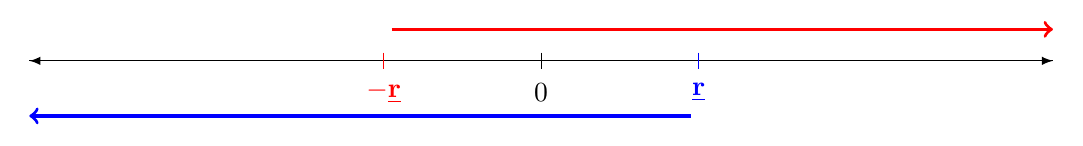
\begin{tikzpicture}
            \draw[latex-] (-6.5,0) -- (6.5,0) ;
            \draw[-latex] (-6.5,0) -- (6.5,0) ;
            \draw[shift={(0,0)},color = black] (0pt,3pt) -- (0pt,-3pt);
            \draw[shift={(0,0)},color = black] (0pt,0pt) -- (0pt,-3pt);
            \node at (0, -0.4) (zero) {0};
            \node[color = blue] at (2, -0.4) (r) {$\underline{\mathbf{r}}$};
            \draw[shift={(2,0)},color = blue] (0pt,3pt) -- (0pt,-3pt);
            \draw[shift={(2,0)},color = blue] (0pt,0pt) -- (0pt,-3pt);
            \draw[<-, shift={(0,-0.7)}, color = blue, very thick] (-6.5,0) -- (1.9,0);
            \node[color = red] at (-2, -0.4) (-r) {$-\underline{\mathbf{r}}$};
            \draw[shift={(-2,0)},color = red] (0pt,3pt) -- (0pt,-3pt);
            \draw[shift={(-2,0)},color = red] (0pt,0pt) -- (0pt,-3pt);
            \draw[->, shift={(0,0.4)}, color = red, very thick] (-1.9,0) -- (6.5,0);
        \end{tikzpicture}
    \end{center}
\end{definition}

From the definition of $-\underline{\mathbf{r}}$, one immediate result is the following.

\begin{proposition}
    $-\underline{\mathbf{r}} \in \mathbb{R}$. (You can kindly use the fact that the set of rational numbers also satisfy the axioms of arithmetics).
\end{proposition}

\begin{proof}
    By taking arbitrary $r \in \underline{\mathbf{r}} \in \mathbb{R}$, and so $-r \in \mathbb{R}$ for all $-r \in - \underline{\mathbf{r}}$.
\end{proof}

\begin{proposition}
    For all $\underline{\mathbf{r}} \in \mathbb{R}, -\underline{\mathbf{r}} + \underline{\mathbf{r}} = \underline{\mathbf{0}}$, where $\underline{\mathbf{0}} = \{ x \in \mathbb{Q} : x < 0 \}$.
\end{proposition}

\begin{proof}
    This result is too tough to prove. Therefore it will not be an exercise.
\end{proof}

We define "multiplication" of Dedekind cuts as follows

\begin{definition}
    For all $\underline{\mathbf{r}}, \underline{\mathbf{s}} \in \mathbb{R}$
    $$\underline{\mathbf{r}} \cdot \underline{\mathbf{s}} = \{ x \in \mathbb{Q} : x < r \cdot s \text{ where }  r \in \underline{\mathbf{r}} \text{ and } s \in \underline{\mathbf{s}} \}$$
    If $\underline{\mathbf{r}} \cdot \underline{\mathbf{s}} \in \mathbb{P}$ then
    $$\underline{\mathbf{r}} \cdot \underline{\mathbf{s}} = \{ p \in \mathbb{Q} : p < r \cdot s \text{ where }  r > 0, r \in \underline{\mathbf{r}} \text{ and } s > 0, s \in \underline{\mathbf{s}} \}$$
\end{definition}

\begin{proposition}
    For all $\underline{\mathbf{r}}, \underline{\mathbf{s}} \in \mathbb{R}, \underline{\mathbf{r}} \cdot \underline{\mathbf{s}} \in \mathbb{R}$ and is another Dedekind cut.
\end{proposition}

\begin{proof}
    This is similar to Proposition \ref{Proposition 1.8.5}. Exercise.
\end{proof}

Since we have proven the commutativity and associativity of Dedekind cuts under addition in Proposition \ref{Proposition 1.8.6}, similarly we can prove the same result under multiplication.

\begin{proposition}
    \begin{itemize}
        \item[(1)] $\underline{\mathbf{r}} \cdot \underline{\mathbf{s}} = \underline{\mathbf{s}} \cdot \underline{\mathbf{r}}$ where they are all Dedekind cuts.
        \item[(2)] $(\underline{\mathbf{r}} \cdot \underline{\mathbf{s}}) \cdot \underline{\mathbf{t}} = \underline{\mathbf{r}} \cdot (\underline{\mathbf{s}} \cdot \underline{\mathbf{t}})$ where they are all Dedekind cuts.
    \end{itemize}
\end{proposition}

\begin{proof}
    Similar to Proposition \ref{Proposition 1.8.6}. Exercise.
\end{proof}

We can also have ordering of Dedekind cuts.

\begin{definition}
    We say that $\underline{\mathbf{r}} < \underline{\mathbf{s}}$ if $\underline{\mathbf{r}} \subset \underline{\mathbf{s}}$, and $\underline{\mathbf{r}} \leq \underline{\mathbf{s}}$ if $\underline{\mathbf{r}} \subseteq \underline{\mathbf{s}}$. \\
    In this case, we can also define \textbf{a positive set of real numbers} be $\mathbb{P} = \{ \underline{\mathbf{r}} \in \mathbb{R}: \underline{\mathbf{0}} < \underline{\mathbf{r}} \}$
\end{definition}

\begin{proposition}
    For all $\underline{\mathbf{r}}, \underline{\mathbf{s}} \in \mathbb{R}, \underline{\mathbf{r}} < \underline{\mathbf{s}} \iff \underline{\mathbf{s}} - \underline{\mathbf{r}} \in \mathbb{P}$
\end{proposition}

\begin{proof}
    Given $\underline{\mathbf{r}}, \underline{\mathbf{s}}, \underline{\mathbf{t}}$, we have $\underline{\mathbf{r}} < \underline{\mathbf{s}} \implies \underline{\mathbf{r}} \subset \underline{\mathbf{s}} \implies \underline{\mathbf{r}} + \underline{\mathbf{t}} < \underline{\mathbf{s}} + \underline{\mathbf{t}}$ (the last step is not that straightforward therefore it would be a good exercise for the readers). \\
    Now, let $\underline{\mathbf{t}} = -\underline{\mathbf{r}}$. We have $\underline{\mathbf{r}} + (- \underline{\mathbf{r}}) < \underline{\mathbf{s}} + (- \underline{\mathbf{r}}) \implies \underline{\mathbf{0}} < \underline{\mathbf{s}} - \underline{\mathbf{r}} \implies \underline{\mathbf{s}} - \underline{\mathbf{r}} \in \mathbb{P}$
\end{proof}

Note that this result is very similar to the one of the axioms we used in ordering of the rationals. In fact, there are much more results that have high similarity and can be proven. This includes following theorems.

\begin{theorem}[Trichotomy]
    For all $\underline{\mathbf{r}} \in \mathbb{R}$
    \begin{itemize}
        \item[(1)] $\underline{\mathbf{r}} = 0$
        \item[(2)] $\underline{\mathbf{r}} \in \mathbb{P}$
        \item[(3)] $-\underline{\mathbf{r}} \in \mathbb{P}$
    \end{itemize}
\end{theorem}

\begin{theorem}[Closure under addition and multiplication]
    For all $\underline{\mathbf{r}}, \underline{\mathbf{s}} \in \mathbb{P}$
    \begin{itemize}
        \item[(1)] $\underline{\mathbf{r}} + \underline{\mathbf{s}} \in \mathbb{P}$
        \item[(2)] $\underline{\mathbf{r}} \cdot \underline{\mathbf{s}} \in \mathbb{P}$
    \end{itemize}
\end{theorem}

Since this is an introduction to Real Analysis, I think this is a good place to end Dedekind cuts. We will be looking at boundedness, supremum/infimum, and density of a set in the next section.

\section{Boundedness, Supremum/Infimum and Density}
We now have already know how to compare two different sets to see whether one is "bigger in size" than the other. What kind of characteristic can we define on a single set (in this case sets contains real numbers)? One thing we like to find is a number that is larger/smaller than any element in the set. Here, we will define the following term.

\begin{definition}
    Given $S \subseteq \mathbb{R}$, we say that M is an \textbf{upperbound} for S if for all $s \in S, s \leq M$. If S has an upperbound, we sometimes say that S is bounded above.\\
    Similarly, we say that m is a \textbf{lowerbound} for S if for all $s \in S, s \geq m$. If S has a lowerbound, we sometimes say that S is bounded below. \\
    We say S is bounded if it is both bounded above and below.
\end{definition}

\begin{example} \label{Example 1.9.2}
    \begin{itemize}
        \item[(1)] 5 is an upperbound for the set $S_{1} = \{ 1, 2, 3, 4 \}$. Note that 4 is also an upperbound. Similarly, 0 and 1 can be the lowerbound of $S_{1}$. 
        \item[(2)] If $S_{2} = (0,1)$, then 1 is an upperbound for $S_{2}$, 0 is an lowerbound for $S_{2}$.
    \end{itemize}
\end{example}

\textbf{Note:} The two example given above clearly shows that the upper/lowerbound may (Example 1) or maynot (Example 2) be in the set. And there are often more than one upper/lowerbound of the same set! \\

We now know some basics understanding of bounded sets. And we are able to give an upper/lowerbound. However, we often know that a set has multiple upper/lowerbounds. What are the upper/lowerbounds that is more interesting and more worth to investigate? This leads us to introduce supremum (least upperbound) and infimum (greatest lower bound).

\begin{definition}
    We say that M is the \textbf{supremum} of S, denoted sup(S), is the least upperbound of S. That is, for any upperbound $\bar{M}, \bar{M} \geq M$.
    Similarly, we say that m is the \textbf{infimmum} of S, denoted inf(S), is the greatest lowerbound of S. That is, for any lowerbound $\bar{m}, \bar{m} \leq m$.
\end{definition}

Back to the Example \ref{Example 1.9.2}, we have that 4 is the supremum, 1 is the infimum of $S_{1}$. And 1 is the supremum, 0 is the infimum of $S_{2}$. This also shows that supremum is not always in the set. Also, there must always be one supremum/infimum (check, and this is an easy proof which directly contradict the definition). \\

Sometimes, we want to find whether supremum exists in a set, but we do not necessarily know (and it is not important to know what are the elements are in the set, this is how Maths is, we typically deals with generic stuff). Then the following gives a important condition for the supremum of a set to exist. This is called the Completeness Axiom, and you can use it without proving it.

\begin{theorem}[Completeness Axiom] \label{Theorem 1.9.4}
    Suppose set S is non-empty and bounded above, then sup(S) exists.
\end{theorem}

\textbf{Note:} Although the non-empty condition of S is pretty intuitive, this condition is typically forgotten frequently by a lot of people. If $S = \emptyset$, then any real number a is an upperbound for S, since $\forall s \in \emptyset, s \leq a$. And there is no supremum for that, since to get a smaller upperbound, we can keep making our a smaller and smaller. \\
Also, completeness Axiom for supremum also works for infimum, as $inf(S) = -sup(-S)$, you can try to prove it.

\begin{proposition}
    If S is non-empty and is bounded above by M = sup(S) $\iff \forall \epsilon > 0, \exists s \in S, \text{ such that } M - \epsilon < s \leq M$. Note that this result also works for infimum. In fact, all the results obtained the Completeness Axiom also works for infimum.
\end{proposition}

\textbf{Note:} we just introduced a new symbol $\epsilon$. In the field of Mathematics, we typically use this symbol to refer any positive real number (typically the very small one). Hence, our argument meant that no matter how close we get to the supremum from the left, we can always find some element in set S that is closer to the supremum. The diagram below also shows the meaning of this proposition.

\begin{center}
    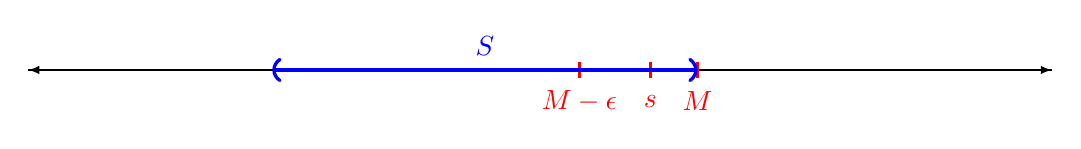
\begin{tikzpicture}
        \draw[latex-] (-6.5,0) -- (6.5,0) ;
        \draw[-latex] (-6.5,0) -- (6.5,0) ;
        \draw[shift={(0.5,0)}, color = red, very thick] (0pt,3pt) -- (0pt,-3pt);
        \draw[shift={(0.5,0)}, color = red, very thick] (0pt,0pt) -- (0pt,-3pt);
        \node[color = red] at (0.5, -0.4) (M-epsilon) {$M-\epsilon$};
        \node[color = red] at (1.4, -0.4) (M-epsilon) {$s$};
        \draw[shift={(1.4,0)},color = red, very thick] (0pt,3pt) -- (0pt,-3pt);
        \draw[shift={(1.4,0)},color = red, very thick] (0pt,0pt) -- (0pt,-3pt);
        \node[color = red] at (2, -0.4) (M) {$M$};
        \node[color = blue] at (-0.7, 0.3) (S) {$S$};
        \draw[shift={(2,0)}, color = red, very thick] (0pt,3pt) -- (0pt,-3pt);
        \draw[shift={(2,0)},color = red, very thick] (0pt,0pt) -- (0pt,-3pt);
        \draw[(-), color = blue, very thick] (-3.4,0) -- (2,0);
    \end{tikzpicture}
\end{center}

\begin{proof}
    ($\Rightarrow$) Suppose M = sup(S), and given $\epsilon > 0$. Suppose for a contradiction that there is no $s \in S$ such tat $M - \epsilon < s \leq M$. That is, $\forall s \in S, s < M - \epsilon$. Then $M - \epsilon$ is an upperbound for S, contradiction that M is the supremum as $M - \epsilon$ is smaller than M. \\
    ($\Leftarrow$) Suppose that $\forall \epsilon > 0, \exists s \in S, M - \epsilon < s \leq M$. Suppose for a contradiction that $M \neq sup(S)$, so that sup(S) < M. Let $\epsilon = M - sup(S) > 0$, and take $s \in S$ such that $M - \epsilon < s \leq M \implies sup(S) < s \leq M$. This contradicts that sup(S) is an upperbound.
\end{proof}

So far we have try to show whether a set is bounded above/below. We haven't show some sets are not, e.g. the set of Natural numbers. This is commonly known as the Archimedean Property.

\begin{theorem}[Archimedean Property]
    $\mathbb{N}$ is not bounded above.
\end{theorem}

\begin{proof}
    Suppose for a contradiction that $\mathbb{N}$ is bounded above. Then by Completeness Axiom (Theorem \ref{Theorem 1.9.4}), $sup(\mathbb{N}$ exists. Then $\forall n \in \mathbb{N}, n \leq sup(\mathbb{N})$, hence $\forall n \in \mathbb{N}, n + 1 \leq sup(\mathbb{N})$, where $n + 1 \in \mathbb{N}$. But then $\forall n \in \mathbb{N}, n \leq sup(\mathbb{N}) - 1$, and $sup(\mathbb{N}) - 1$ is an upper bound, contradiction. Thus $\mathbb{N}$ is not bounded above.
\end{proof}

This gives an immediate corollary.

\begin{corollary} \label{Corollary 1.9.7}
    If $\epsilon > 0$, $\exists N \in \mathbb{N}$ such that $\frac{1}{N} < \epsilon$.
\end{corollary}

\begin{proof}
    If not, then $\forall N \in \mathbb{N}, \frac{1}{N} < \epsilon \implies \forall N \in \mathbb{N}, N < \frac{1}{\epsilon}$ showing that $\frac{1}{\epsilon}$ is an upperbound for $\mathbb{N}$, contradiction.
\end{proof}

Lastly, I would like to introduce density of a set. These are not relevant to boundedness, but these are also important to know before covering the actual Real Analysis of functions. In fact, this would be our last thing to cover before diving into the Real Analysis of functions.

\begin{definition}
    A set $S \subseteq \mathbb{R}$ is \textbf{dense} in $\mathbb{R}$ if $\forall a < b, (a, b) \cap S \neq \emptyset$. \\
    In other words, this meant that for any open interval (no matter how small it is), we can always find a number within this interval that is also an element in D.
\end{definition}

One of the pretty "intuitive" result is the density of the rationals.

\begin{proposition} \label{Proposition 1.9.9}
    $\mathbb{Q}$ is dense in $\mathbb{R}$.
\end{proposition}

\begin{proof}
    Suppose for a contradiction that such (a, b) exists. By Corollary \ref{Corollary 1.9.7}, we can choose $N \in \mathbb{N}$ such that $\frac{1}{N} < b - a$. \\
    Now, define S as follows
    $$S = \{ \frac{m}{N} : m \in \mathbb{Z} \} \subseteq \mathbb{Q}$$
    By assumption, $S \cap (a, b) = \emptyset$. Let $M \in \mathbb{Z}$ be the largest integer such that $\frac{M}{N} < a$. Note that M is defined as there exists an $M \in \left \lfloor{a}\right \rfloor N < M < \left \lceil{a}\right \rceil N$, where $\left \lceil{a}\right \rceil$ is the floor function of a, the greatest integer that is smaller or equal to a. And $\left \lceil{a}\right \rceil N$ is the ceiling function, the smallest integer that is greater or equal to a. \\
    Now, we have that $\frac{M + 1}{N} > b$, since $S \cap (a, b) = \emptyset$. But we have that $b - a < \frac{M + 1}{N} - \frac{M}{N} = \frac{1}{N} < b - a$, contradiction.
\end{proof}

Similarly, we can make a similar argument for irrational numbers.

\begin{proposition}
    $\mathbb{R}\backslash\mathbb{Q}$ is dense in $\mathbb{R}$
\end{proposition}

\begin{proof}
    By Proposition \ref{Proposition 1.9.9}, there exists an $s_{1} \in (a, b)$ where $s_{1} \in \mathbb{Q}$. Similarly, 
    there exists an $s_{2} in (s_{1}, b)$ where $s_{2} \in \mathbb{Q}$. Now, we define 
    $$s = s_{1} + \frac{s_{2} - s_{1}}{\sqrt{2}}$$
    And we have that $s \in (s_{1}, s_{2}) \subseteq (a, b)$ and s is irrational.
\end{proof}

\chapter{Limits and Continuity}
Starting from this chapter, we are going to investigate real functions thoroughly. I hope this is not a new term to everyone, all of you can give some examples of a real function. 

\begin{itemize}
    \item $f : \mathbb{R} \rightarrow \mathbb{R}$ where $f(x) = x^{2}$ is a real function.
    \item $g : \mathbb{R} \rightarrow \mathbb{R}$ where $g(x) = \frac{x^{2} + 2}{x^{3} - 2x + 1}$ is a real function.
    \item $h : \mathbb{R} \rightarrow \mathbb{R}$ where $g(x) = \frac{\sin(e^{x})}{x^{2}}$ is a real function.
\end{itemize}

If you try to plot these on any graphing software (desmos, or whatever), you will see that the curves are smooth (if you know, they are both continuous and differentiable), which is pretty nice. However, what if I tell you now that these functions are only a tiny part of all the real functions, and what we want to do is to also investigate other functions that are not that nice. What does that mean? It means that not all the real functions are very well-behaved. Most functions are not smooth (not differentiable and/or not continuous). In fact, there are a lot of functions that are so badly behaved that it is everyone not continuous and/or not differentiable. As a motivating problem, I will like to let you think of this question.

{\centering \textbf{What are the examples of functions that is absolutely discontinuous or not differentiable.}}

Even if you cannot come up with examples. That is completely fine. Remember this question and continue reading, eventually this question will be answered in some part of this book.

We will be first dealing with the formal definition of some familiar terms such as the limits and continuity. We will also be looking at how we can formally define asymptotes. This will then be followed by some more unfamiliar topics such as uniform continuity and the three hard theorems.


\section{Limit}

An informal way to think of a limit where x approaching c is the value of $f(x)$ when x approaching c. This is actually logically correct, but we cannot rely on this criterion to find the limit as for the most cases, it only works on function that is well-behaved. In fact, we will try to find the limit of some badly behave functions but we can't find it if we use our informal criterion. Before introducing the formal definition of a limit, I would like to bring your attention to the following example.
\begin{center}
    \begin{tikzpicture}
        \begin{axis}
            [
            axis lines = left,
            xlabel = \(x\),
            ylabel = \(f(x)\),
            xmin = -3,
            xmax = 2,
            ymin = -5,
            ymax = 9,
            ]
            \addplot[color = blue, very thick, samples = 100] {x^3 + 3 * x^2 + 3 * x + 2};
            \draw [densely dashed, very thick, blue] (-1, 3) -- (-1, -5);
            \draw [color = blue, fill = white, very thick] (-1,1) circle [radius=2pt];
            \draw [color = blue, fill = blue, very thick] (-1,3) circle [radius=2pt];
            \addlegendentry {\(x^3 + 3x^2 + 3x + 2\)}
        \end{axis}
    \end{tikzpicture}
\end{center}

From the graph, suppose that we have the function that is badly behave at $x = -1$, where $f(-1) = 3$, but I guess everyone would agree that if f is well-behaved then $f(-1)$ should be at 1. What we would like to do is to determine what f does when $x = -1$ if we ignore the bad point at $x = -1$, meaning, we don't care what is the actual value of f(0). In other words, we would like to find what value $f(-1)$ should be by looking at how $f(x)$ behaves when x is around -1 (but not equal -1). This gives the following definition of a limit.

\begin{definition}
    Given set $S \subseteq \mathbb{R}$, suppose $f : S \rightarrow \mathbb{R}$ and $c \in S$. We say that
    $$\lim_{x \rightarrow c} f(x) = L$$
    for some $L \in \mathbb{R}$ if
    $$\forall \epsilon > 0, \exists \delta > 0, \text{ s.t. } \forall x \in \mathbb{R}, 0 < |x - c| < \delta \implies |f(x) - L| < \epsilon$$
    In this case, the limit of $f(x)$ when x approaches c is L.
\end{definition}

This might be your first time seeing such a long Maths expression. Don't worry, I will now try to thoroughly explain this and hope that you will understand what each of these symbols mean. \\

First I feel that the absolute value inside the Maths expression is a bit annoying. Thus, I will now change the definition into the following.

$$\forall \epsilon > 0, \exists \delta > 0, \text{ s.t. } \forall x \in \mathbb{R}, x \in (c - \delta, c) \cup (c, c + \delta) \implies f(x) \in (L - \epsilon, L + \epsilon)$$
I am sure you already know what $\epsilon$ is (if you can't remember, it is a positive, typically small, number). Note that in this definition $x \in (c - \delta, c) \cup (c, c + \delta)$ basically means that the value of x around c within a distance $\delta$, and similarly $f(x) \in (L - \epsilon, L + \epsilon)$ means the value of $f(x)$ is around L within the distance $\epsilon$. \\

We think that $\lim_{x \rightarrow c} f(x) = L$, if for any value of $\epsilon > 0$, within the range of $(L - \epsilon, L + \epsilon)$, there is always a value $\delta$, such that any value of x around c (not including c) within the distance $\delta$, the value of $f(x)$ for x within such interval is always around L within the distance $\epsilon$. And this is true for any value of positive number $\epsilon$ (no matter how small it is). Refer back to the same example, we can now try to understand how this definition works graphically.

\begin{center}
    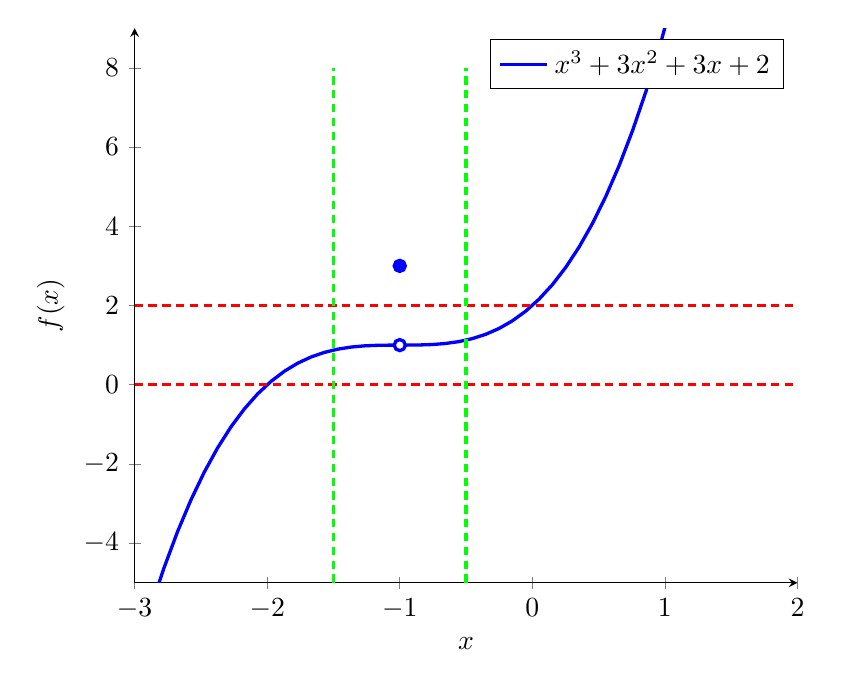
\begin{tikzpicture}
        \begin{axis}
            [
            axis lines = left,
            xlabel = \(x\),
            ylabel = \(f(x)\),
            xmin = -3,
            xmax = 2,
            ymin = -5,
            ymax = 9,
            ]
            \addplot[color = blue, very thick, samples = 100] {x^3 + 3 * x^2 + 3 * x + 2};
            \draw [densely dashed, very thick, red] (-3, 0) -- (2, 0);
            \draw [densely dashed, very thick, red] (-3, 2) -- (2, 2);
            \draw [densely dashed, very thick, green] (-1.5, -5) -- (-1.5, 8);
            \draw [densely dashed, very thick, green] (-0.5, -5) -- (-0.5, 8);
            \draw [color = blue, fill = white, very thick] (-1,1) circle [radius=2pt];
            \draw [color = blue, fill = blue, very thick] (-1,3) circle [radius=2pt];
            \addlegendentry {\(x^3 + 3x^2 + 3x + 2\)}
        \end{axis}
    \end{tikzpicture}
\end{center}

It can be seen that in this situation, we have chosen our $\epsilon = 1$, where we found a value of $\delta$ such that for all x within the interval of $(c - \delta, c + \delta)$ excluding c, all the f(x) stays within the interval of $(L - 1, L + 1)$. Note that if a value of $\delta$ works, any smaller value of $\delta$ also works. \\
We now know that the limit satisfy the definition if $\epsilon = 1$. However, we need to show that the defintion is satisfied for all $\epsilon > 0$. In this case, we cannot prove such statement by generating lots of graphs (no matter how many values of $\epsilon > 0$ we always miss some $\epsilon$ value. Therefore, we need to use a different strategy to prove it. I will now give you some examples.

\begin{example} \label{Example 2.1.2}
    Show that $\lim_{x \rightarrow 2} (7x + 3) = 17$
\end{example}

\begin{proof}
    Plug in $c = 2,f(x) = 7x + 3 \text{ and } L = 17$, We are trying to show that 
    $$\forall \epsilon > 0, \exists \delta > 0, \text{ s.t. } \forall x \in \mathbb{R}, 0 < |x - 2| < \delta, |7x - 14| < \epsilon$$
    We have $|7x - 14| < \epsilon \implies 7|x - 2| < \epsilon \implies |x - 2| < \frac{\epsilon}{7}$. Since $|x - 2| < \delta$, we can pick $\delta = \frac{\epsilon}{7}$ such that
    $$|f(x) - L| = |7x - 14| = 7|x - 2| < 7 \frac{\epsilon}{7} = \epsilon$$
\end{proof}

You might be having trouble understanding what is going on right now. I will try to explain these meaning. Note that in proving such statement is true, we need to prove that our definition of a limit is true. And by our definition, we are given any value of $\epsilon$, and we need to try to show that for any $\epsilon$, there is always a value of $\delta$ such that this holds. Many students start by thinking about epsilon and this exactly not a correct way. As epsilon is arbitrary (the value varies), we can't tell a lot of information from the epsilon. Instead, what we should focus on is the value of $\delta$. We want to find an expression of the value of delta such that it works for all epsilon. This can be done by thinking that the value of delta depends on the value of the epsilon (of which is usually the case). Therefore, in my previous example, I found that if I make $\delta = \frac{\epsilon}{7}$, the definition holds for all epsilon. In fact, the majority part of the proof is just, find the value of the delta, and prove that it works for all epsilon. \\

Finding the value of delta isn't an easy task, it is hard to come up a number that satisfies for all epsilon, especially this is your first time experience this $\epsilon-\delta$ stuff. I would recommend to first work backwards (just like what I did in Example \ref{Example 2.1.2}, all the work before noticing that $\delta = \frac{\epsilon}{7}$ is my rough work, where I substituted all my values of c, f(x) and L. Then I tried to write $|f(x) - L|$ in some form of $|x - c|$ so I am able to write delta in terms of some value of epsilon. Here is another example,

\begin{example}
    Show that $\lim_{x \rightarrow 4} 3 - 2x = -5$
\end{example}

\begin{proof}
    Plug in $c = 2,f(x) = 7x + 3 \text{ and } L = 17$, We are trying to show that 
    $$\forall \epsilon > 0, \exists \delta > 0, \text{ s.t. } \forall x \in \mathbb{R}, 0 < |x - 4| < \delta, |8 - 2x| < \epsilon$$
    We have $|8 - 2x| < \epsilon \implies 2|x - 4| < \epsilon \implies |x - 4| < \frac{\epsilon}{4}$. Since $|x - 4| < \delta$, we can pick $\delta = \frac{\epsilon}{2}$ such that
    $$|f(x) - L| = |8 - 2x| = 2|x - 4| < 2 \frac{\epsilon}{2} = \epsilon$$
\end{proof}

\begin{example}
    \begin{itemize}
        \item[(1)] $\forall c \in \mathbb{R}, \lim_{x \rightarrow c} k = k$
        \item[(2)] $\forall c \in \mathbb{R}, \lim_{x \rightarrow c} x = c$
        \item[(3)] $\forall a, b, c \in \mathbb{R}, a \neq 0, \lim_{x \rightarrow c} ax + b = ac + b$.
    \end{itemize}
\end{example}

\begin{proof}
    Exercise.
\end{proof}

\section{One-Sided Limits}
\section{Vertical Asymptotes}
\section{Horizontal Asymptotes}
\section{Propositions of Limit}
\section{Continuity}
\section{Propositions of Continuity}
\section{Uniform Continuity}
\section{Three Hard Theorems}

\chapter{Differentiation}
\section{Definition of Derivatives}
\section{Power, Product, Quotient, Chain Rule}
\section{Inverse Function Theorem}
\section{Mean Value Theorem}
\section{L'Hopital's Rule}

\chapter{Integration}
\section{Partitions and Riemann Sums}
\section{Darboux Sums and Integrability}
\section{Sufficient Conditions of Integrability}
\section{Jordan Measure}
\section{Anti-derivatives}
\section{Fundamental Theorem of Calculus}
\section{Integration Techniques}
\section{Logarithms and Exponentials}
\section{Improper Integrals - Unbounded Intervals}
\section{Improper Integrals - Unbounded Functions}

\chapter{Sequences and Series}
\section{Sequences and Subsequences}
\section{Convergent Sequences}
\section{Series}
\section{Convergent Series}
\section{Sequences of Functions and Pointwise Convergence}
\section{Uniform Convergence}
\section{Series of Functions}
\section{Polynomial Approximation}
\section{Power Series}
\section{Taylor Series}


\begin{definition}

Given a function $f$, L is a limit when $x=c$ is defined as 
$$\forall\epsilon>0, \exists\delta>0 \ s.t. \ \forall x\in\mathbb{R}, 0<|x-c|<\delta \Rightarrow |f(x)-L|<\epsilon$$
We can write this as
$$\lim_{x\rightarrow c}f(x)=L$$ 
\end{definition}

\begin{example}
Define $f : \mathbb{R} \rightarrow \mathbb{R}$ by $f(x) = 2x + 1$, prove that $$\lim_{x \rightarrow 3}f(x) = 7$$
\begin{proof}
Let $\epsilon > 0$ be given, define $\delta = \frac{\epsilon}{2}$
We have
\begin{align*}
|x-3| < \epsilon/2 & \Rightarrow  2|x-3| < \epsilon\\
&\Rightarrow  |2x-6| < \epsilon\\
&\Rightarrow  |(2x+1)-7| < \epsilon\\
&\Rightarrow  |f(x)-L| < \epsilon
\end{align*}
\end{proof}
\end{example}

\begin{definition}
Given a function $f$, we say that f is continuous at point $c$ when 
$$\lim_{x\rightarrow c}f(x)=f(c)$$ 
that is
$$\forall\epsilon>0, \exists\delta>0 s.t. \forall x\in\mathbb{R}, |x-c|<\delta \Rightarrow |f(x)-f(c)|<\epsilon$$
\end{definition}
From what we have
\begin{align*}
&\frac{ax + b}{2x + 4} = 4\\
\Rightarrow \ & ax + b = 8x + 16\\
\Rightarrow \ & a = 8, b = 16\\  
\end{align*}

\begin{theorem}[Baby Intermediate Value Theorem]
Suppose $f$ is continuous on $[a,b]$ with $f(a)<0$ and $f(b)>0$, then there exists some $c \in [a,b]$ such that $f(c) = 0$
\begin{proof}
Exercise.
\end{proof}
\begin{equation*}
SMB_{food}=
    \begin{cases}
        60 - 2Q & \text{if } x \in [10, 20]\\
        20 - Q & \text{if } x \in [0, 10)\\
        0 & \text{otherwise}
    \end{cases}
\end{equation*}
\end{theorem}
\begin{center}
\begin{tabular}{|c|c|c|c|}
    \hline
    a &b&c&d  \\\hline
    a &b&c&d  \\\hline
    a &b&c&dlskdjnflks  \\\hline
    a &b&c&d  \\\hline
\end{tabular}
\\
\begin{center}
\begin{tabular}{|m{2cm}|m{2cm}|m{2cm}|m{3cm}|}
\hline
& & \multicolumn{2}{|c|}{Player B} \\\hline
& & Advertise & Not advertise \\\hline
\multirow{4}{4em}{Player A} & \multirow{2}{4em}{Advertise} & A: + 100 & A: + 200\\
& & B: + 100 & B: + 0\\\hline
& \multirow{2}{4em}{Not advertise} & A: + 0 & A: + 0\\
& & B: + 200 & B: + 0\\\hline
\end{tabular}
\end{center}
\end{center}
\end{document}
